%To compile as handout, use
%pdflatex "\def\ishandout{1} \input{filename.tex}"
%Defaults to non-handout mode (with slide reveals)
\ifdefined\ishandout
  \documentclass[handout]{beamer}
\else
  \documentclass{beamer}
\fi
 
\usepackage{econ103slides} 

\date{Lecture \# 4}
\begin{document} 


%%%%%%%%%%%%%%%%%%%%%%%%%%%%%%%%%%%%%%%%

\begin{frame}[plain]
	\titlepage 
	

\end{frame} 
%%%%%%%%%%%%%%%%%%%%%%%%%%%%%%%%%%%%%%%%
\begin{frame}

\begin{center}
 \Huge Introduction to Regression
\end{center}

\end{frame}
%%%%%%%%%%%%%%%%%%%%%%%%%%%%%%%%%%%%%%%%
%\begin{frame}
%\frametitle{How to fairly account for missing midterm score?}
%	\begin{itemize}
%		\item In my first semester at Penn, several students missed Midterm 2 because of illness so I decided to up-weight their finals. 
%		\item Problem: Midterm 2 turned out easier than Midterm 1 and this put the students who had missed the second midterm at a disadvantage when I curved the class.
%	\item In order to correct for this, I needed a way to \emph{\alert{fill in}} a score for the missing midterm.
%	\item How could I do this fairly?\pause
%		\begin{itemize}
%			\item Just fill in mean score on second exam?\pause
%			\item Use performance on first midterm to predict?
%		\end{itemize}
%\end{itemize}
%
%\end{frame}
%
%%%%%%%%%%%%%%%%%%%%%%%%%%%%%%%%%%%%%%%%%
%\begin{frame}
%\frametitle{Data for students who took both midterms:}
%\begin{figure}
%	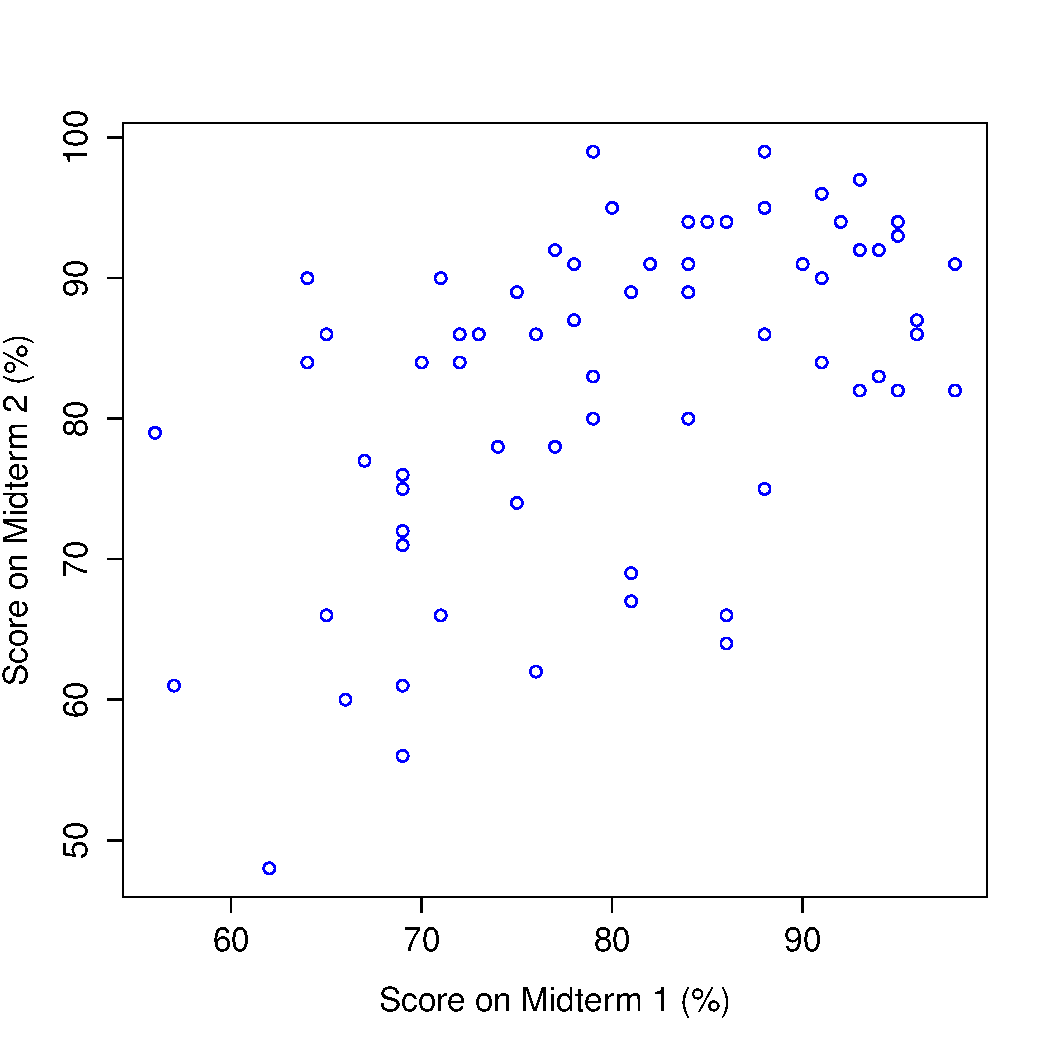
\includegraphics[scale = 0.48]{./images/midterms0}
%\end{figure}
%\end{frame}
%%%%%%%%%%%%%%%%%%%%%%%%%%%%%%%%%%%%%%%%%
\begin{frame}
\frametitle{Predict Second Midterm given 81 on First \hfill 
\includegraphics[scale = 0.05]{./images/clicker} }
\begin{figure}
	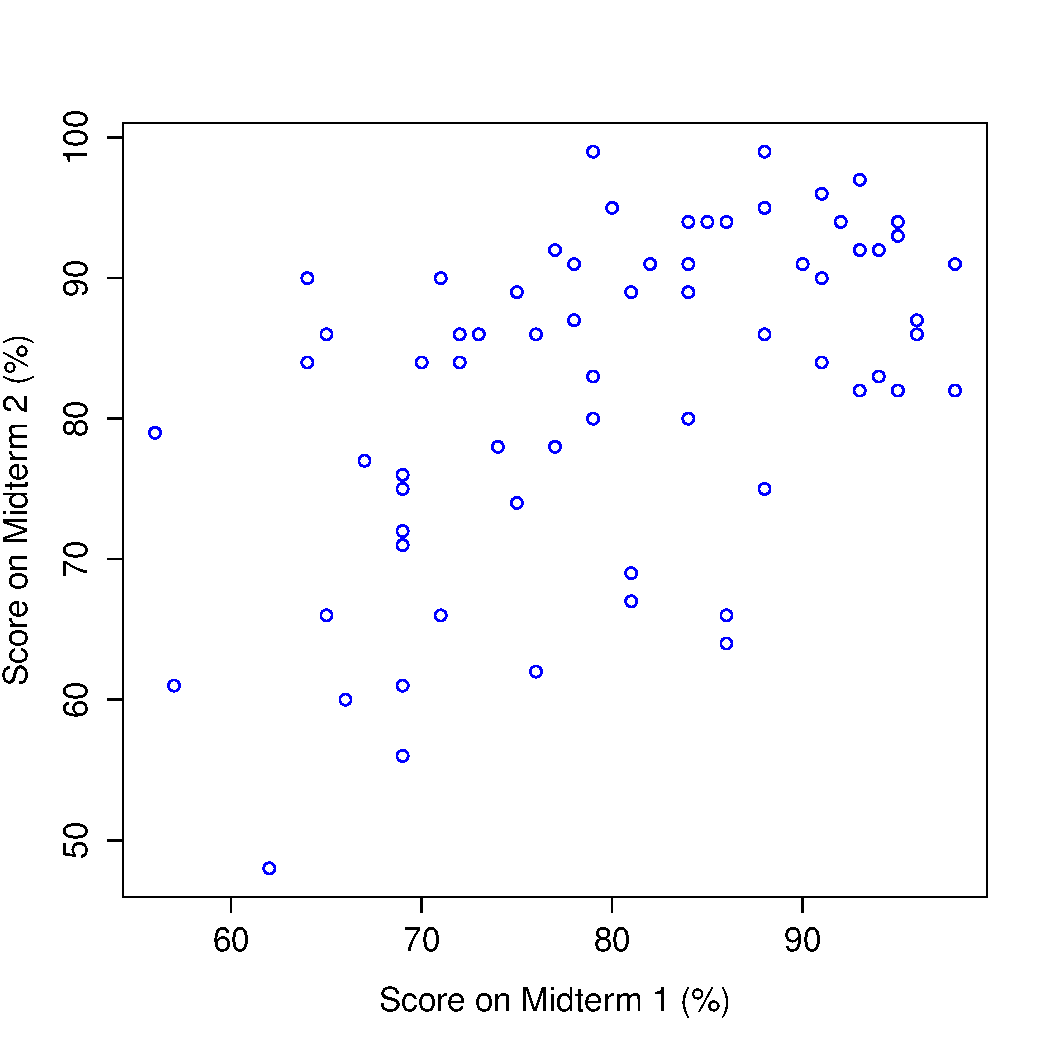
\includegraphics[scale = 0.48]{./images/midterms0}
\end{figure}
\end{frame}
%%%%%%%%%%%%%%%%%%%%%%%%%%%%%%%%%%%%%%%%
\begin{frame}
\frametitle{Predict Second Midterm given 81 on First}
\begin{figure}
	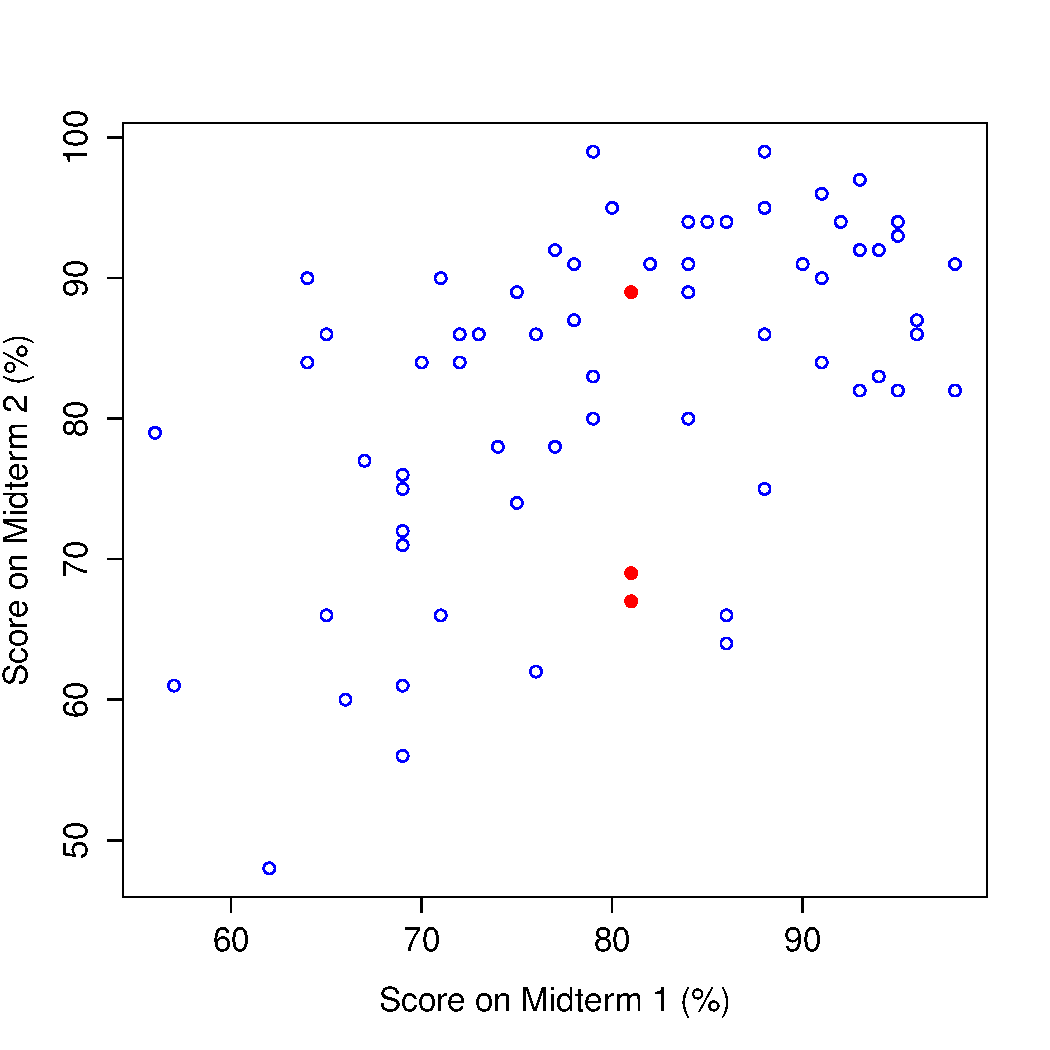
\includegraphics[scale = 0.48]{./images/midterms1}
\end{figure}
\end{frame}
%%%%%%%%%%%%%%%%%%%%%%%%%%%%%%%%%%%%%%%%
\begin{frame}
\frametitle{Predict Second Midterm given 81 on First}
\begin{figure}
	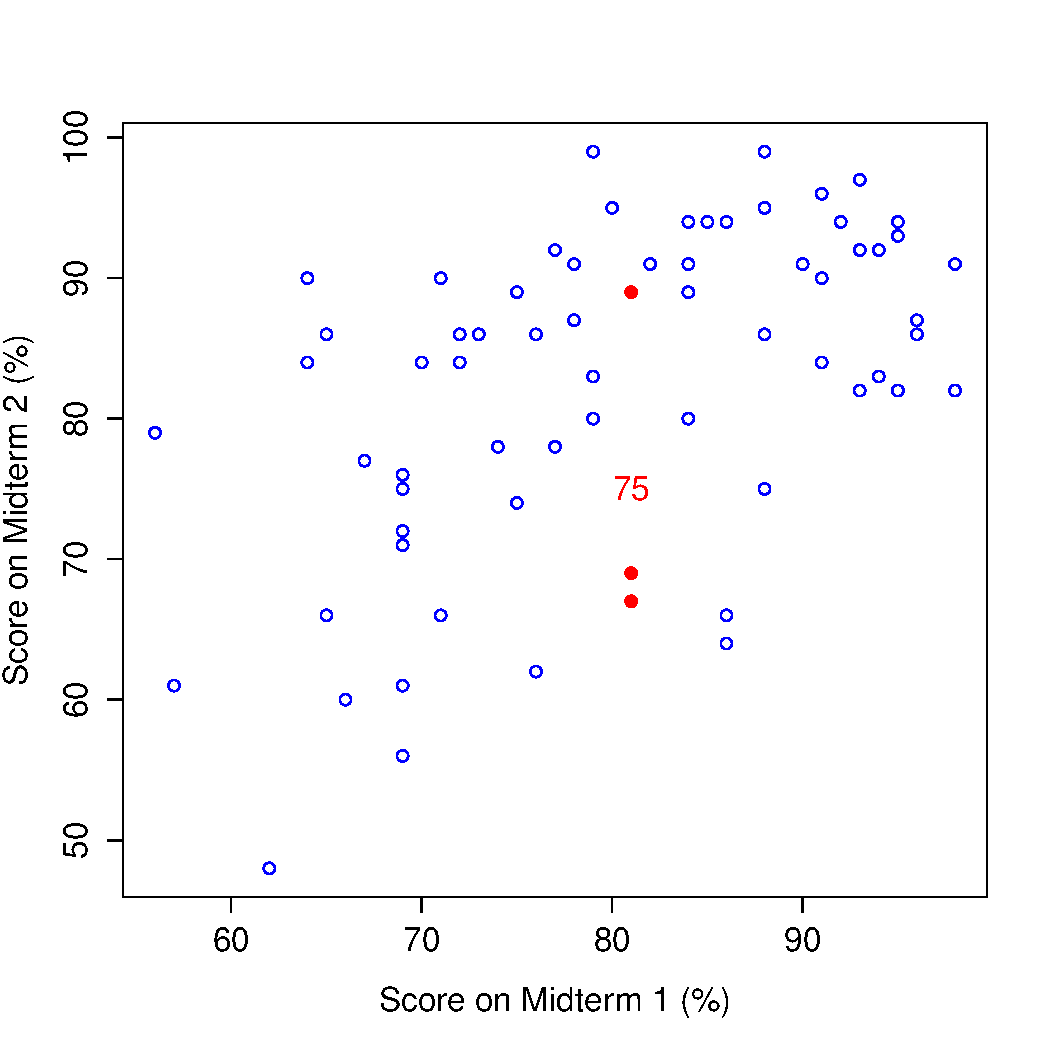
\includegraphics[scale = 0.48]{./images/midterms2}
\end{figure}
\end{frame}
%%%%%%%%%%%%%%%%%%%%%%%%%%%%%%%%%%%%%%%%
\begin{frame}
\frametitle{But if they'd only gotten 79 we'd predict higher?!}
\begin{figure}
	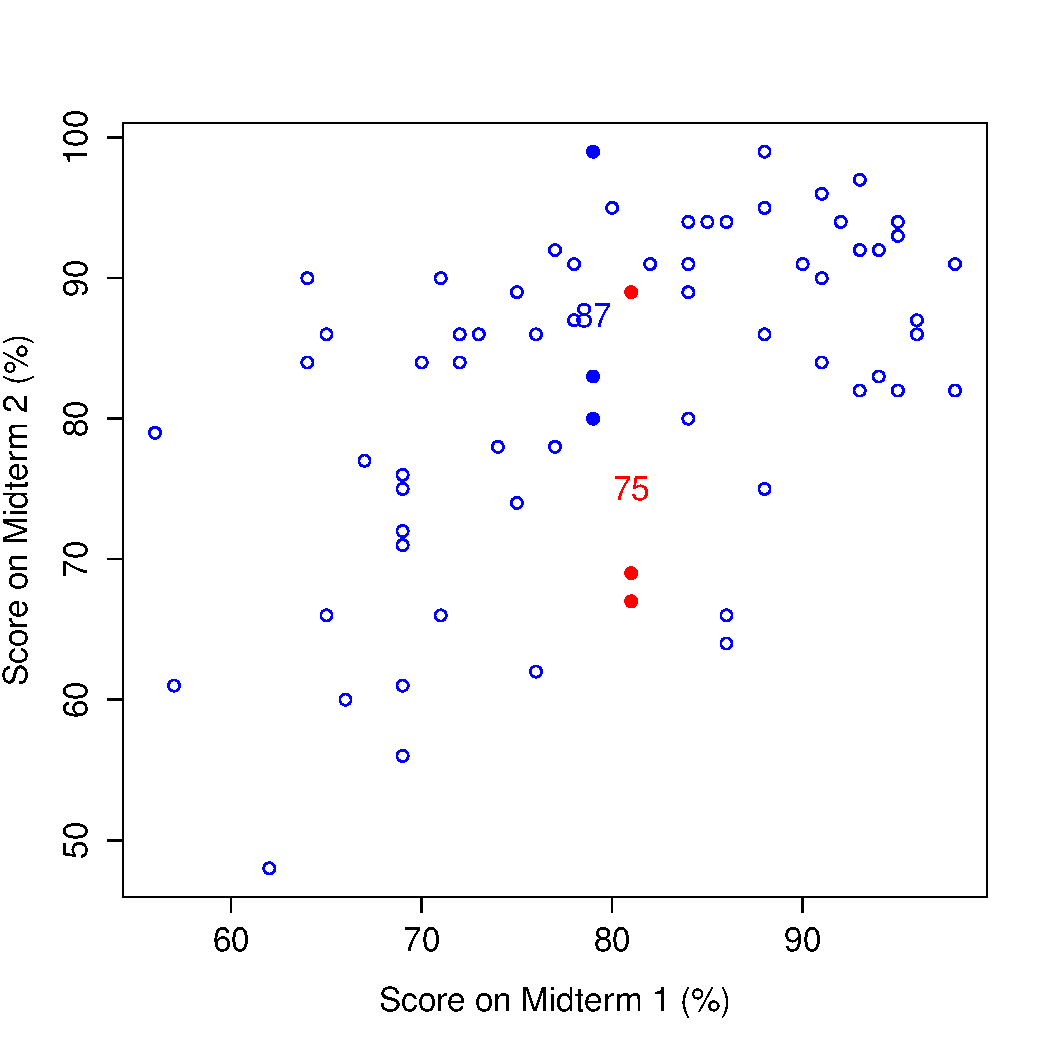
\includegraphics[scale = 0.48]{./images/midterms3}
\end{figure}
\end{frame}
%%%%%%%%%%%%%%%%%%%%%%%%%%%%%%%%%%%%%%%%
\begin{frame}
\frametitle{No one who took both exams got 89 on the first!}
\begin{figure}
	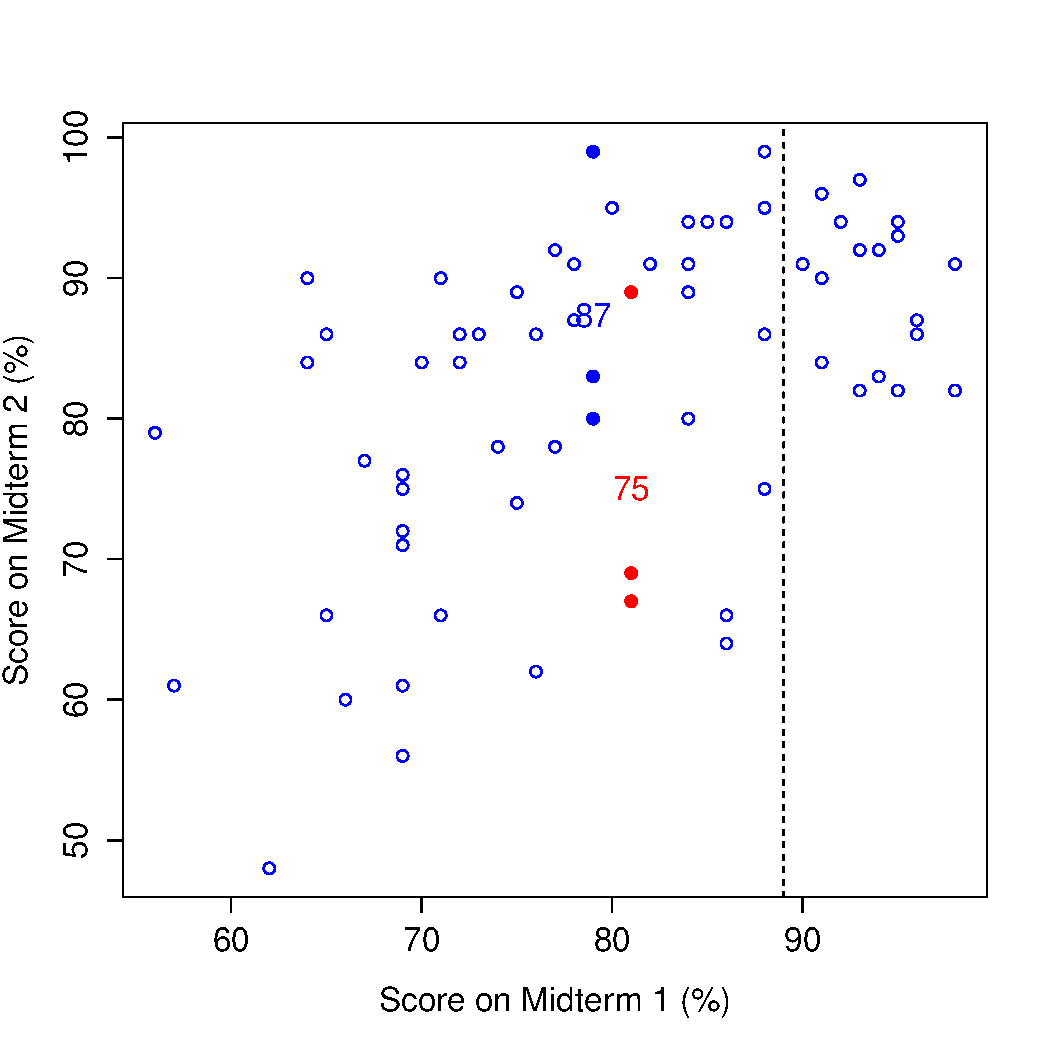
\includegraphics[scale = 0.48]{./images/midterms4}
\end{figure}
\end{frame}
%%%%%%%%%%%%%%%%%%%%%%%%%%%%%%%%%%%%%%%%
\begin{frame}
\frametitle{Regression: ``Best Fitting'' Line Through Cloud of Points}
\begin{figure}
	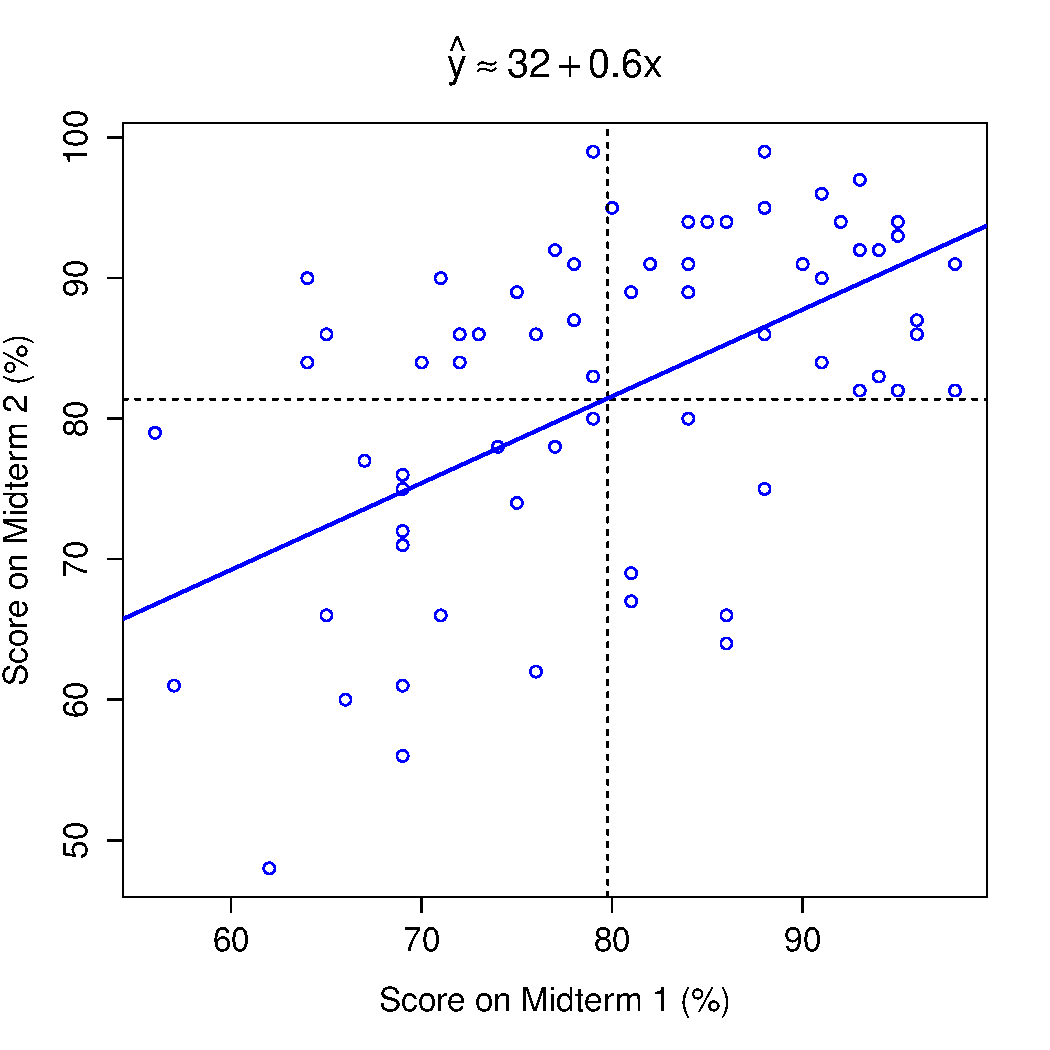
\includegraphics[scale = 0.48]{./images/midterms5}
\end{figure}
\end{frame}
%%%%%%%%%%%%%%%%%%%%%%%%%%%%%%%%%%%%%%%%

\begin{frame}

\centering \Huge Fitting a Line by Eye


\end{frame}

%%%%%%%%%%%%%%%%%%%%%%%%%%%%%%%%%%%%%%%%

\begin{frame}

\centering{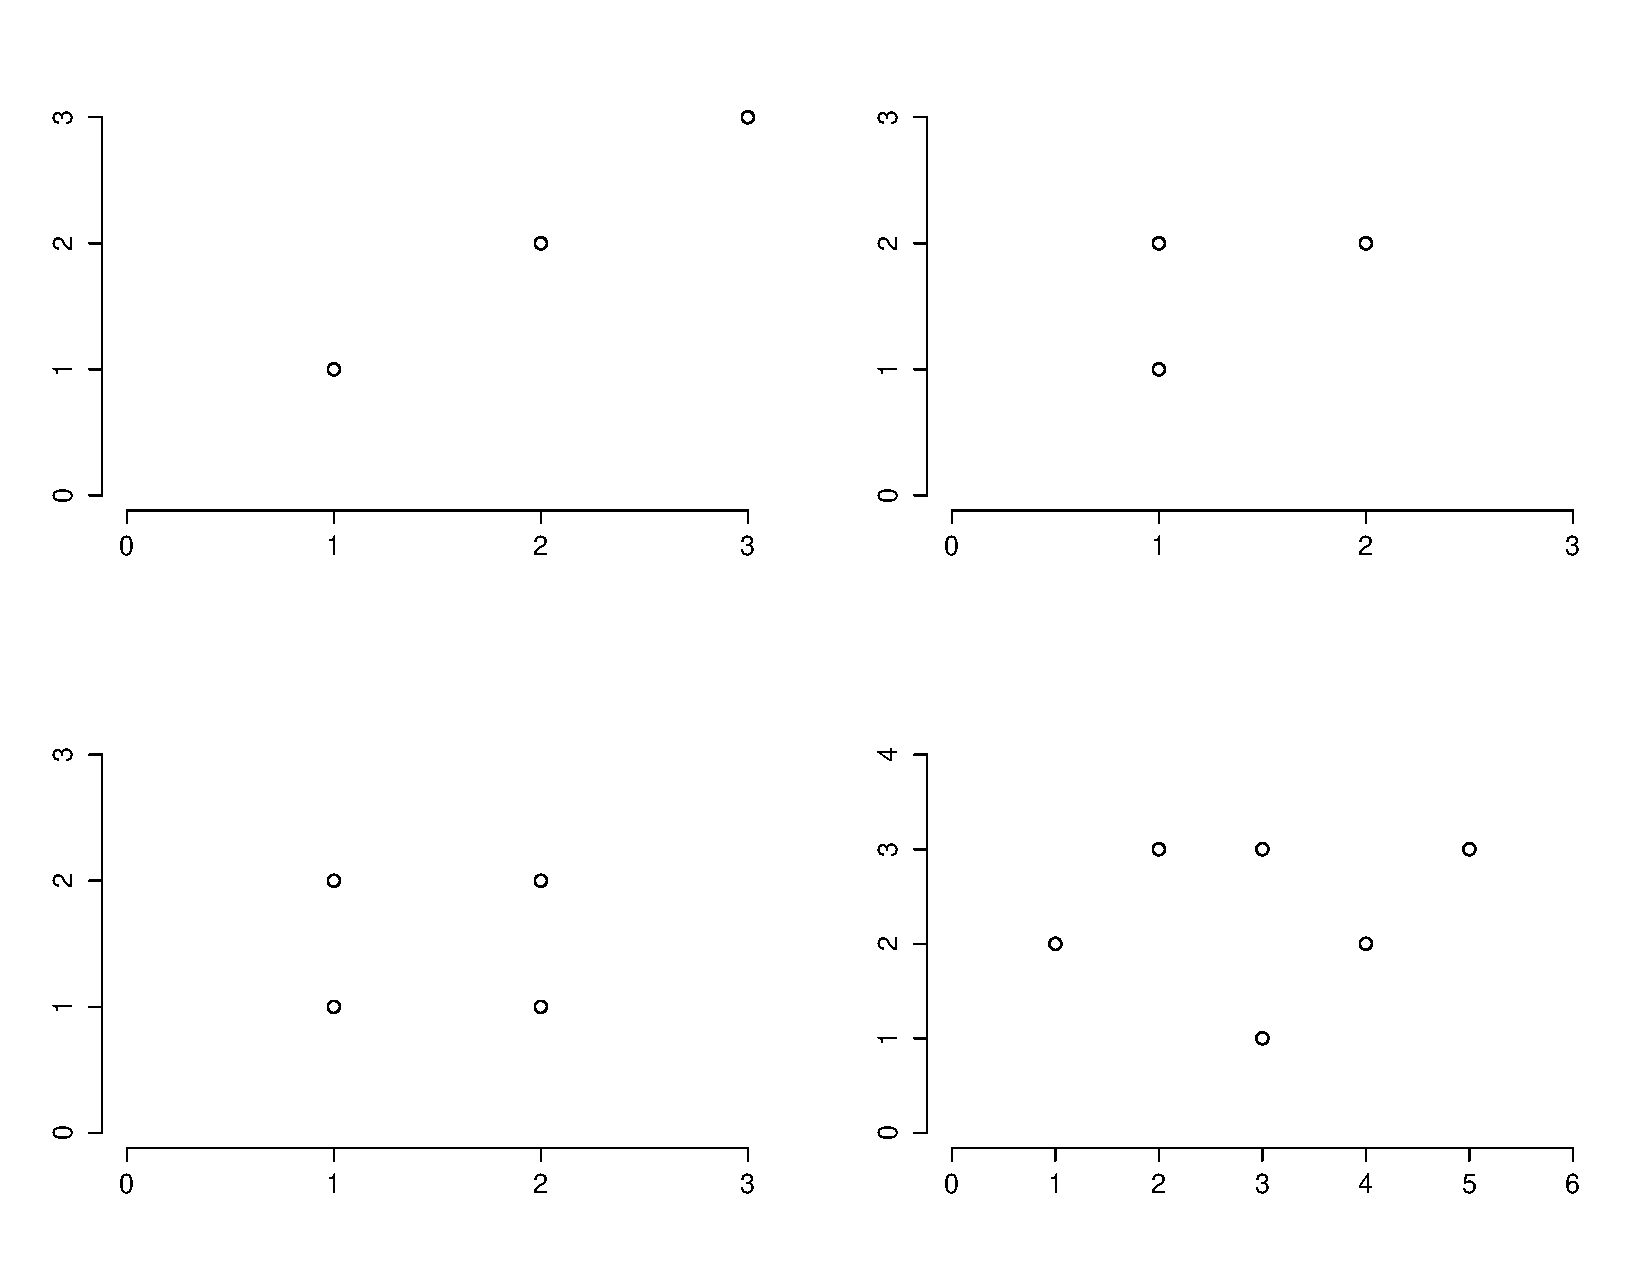
\includegraphics[scale = 0.4]{./images/Gelman_example1}}


\end{frame}

%%%%%%%%%%%%%%%%%%%%%%%%%%%%%%%%%%%%%%%%

\begin{frame}

\centering{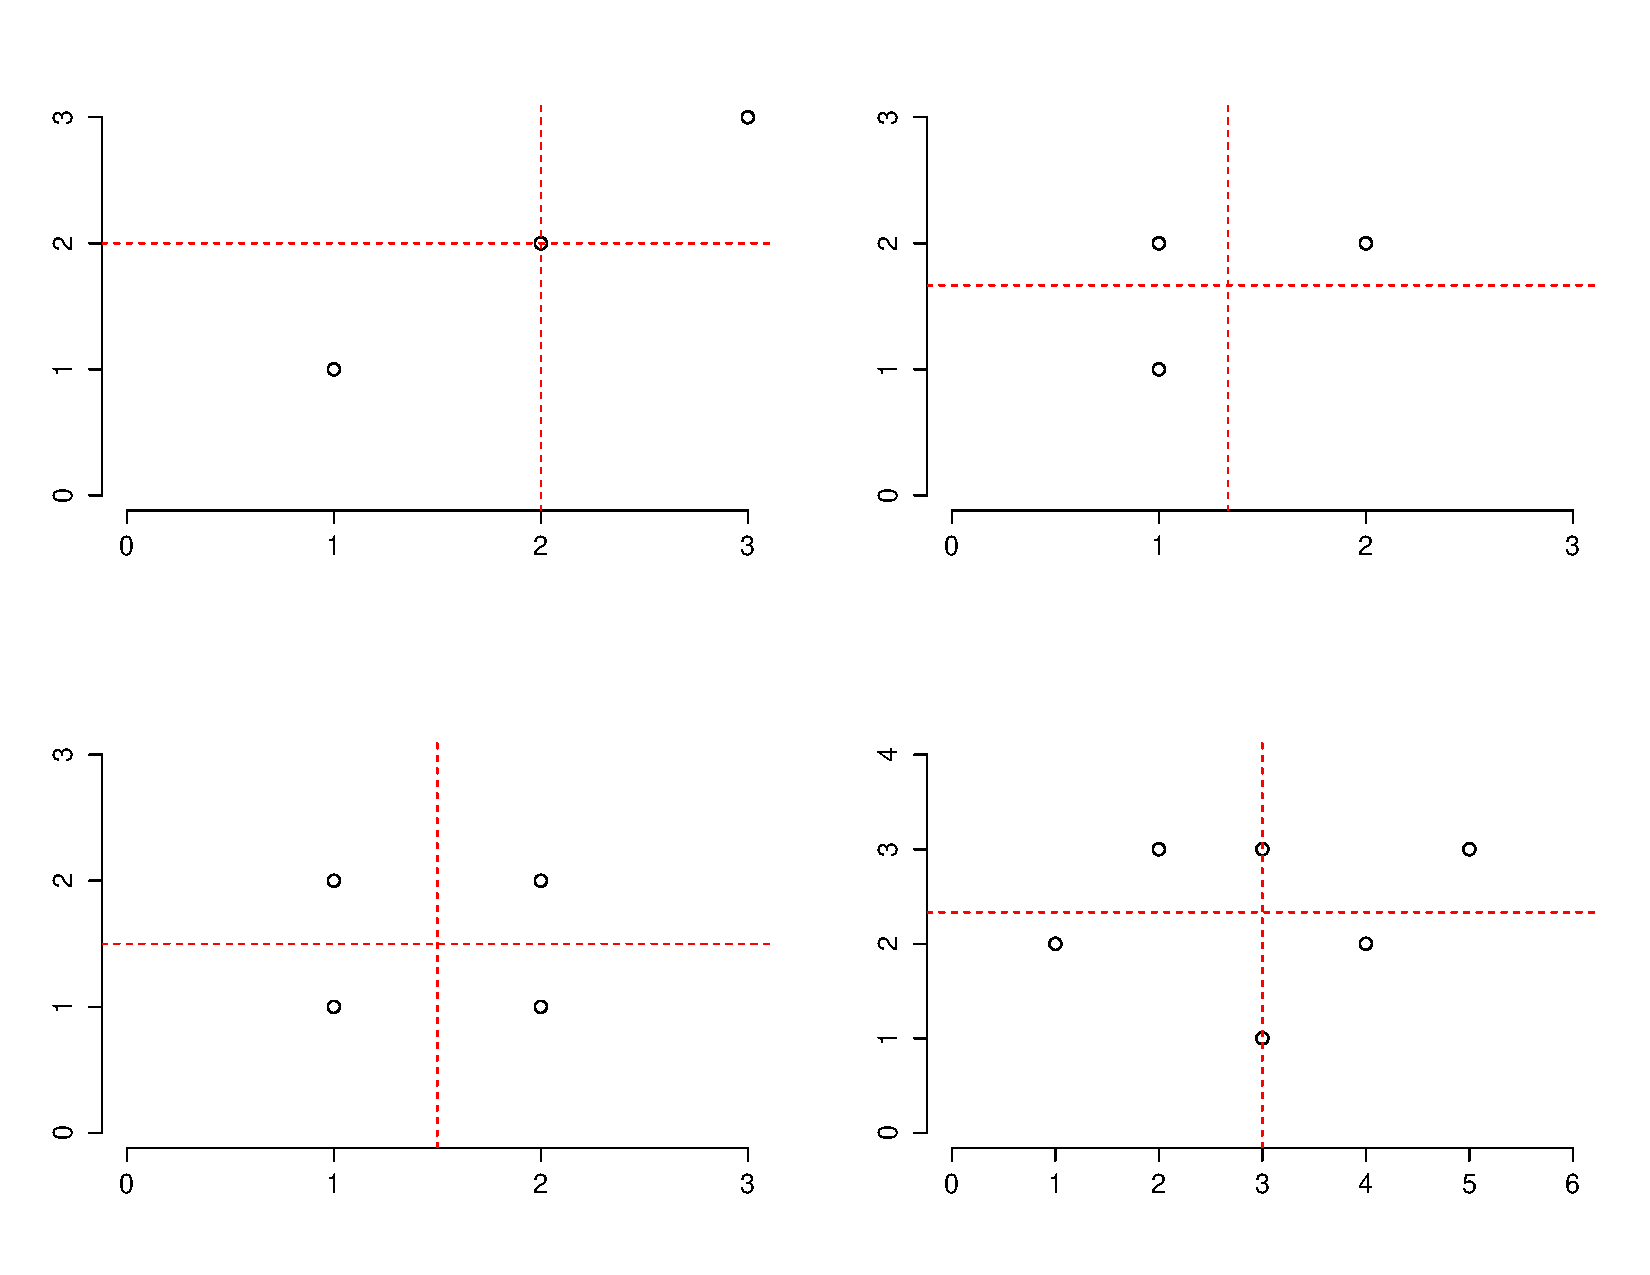
\includegraphics[scale = 0.4]{./images/Gelman_example2}}


\end{frame}

%%%%%%%%%%%%%%%%%%%%%%%%%%%%%%%%%%%%%%%%

\begin{frame}

\centering{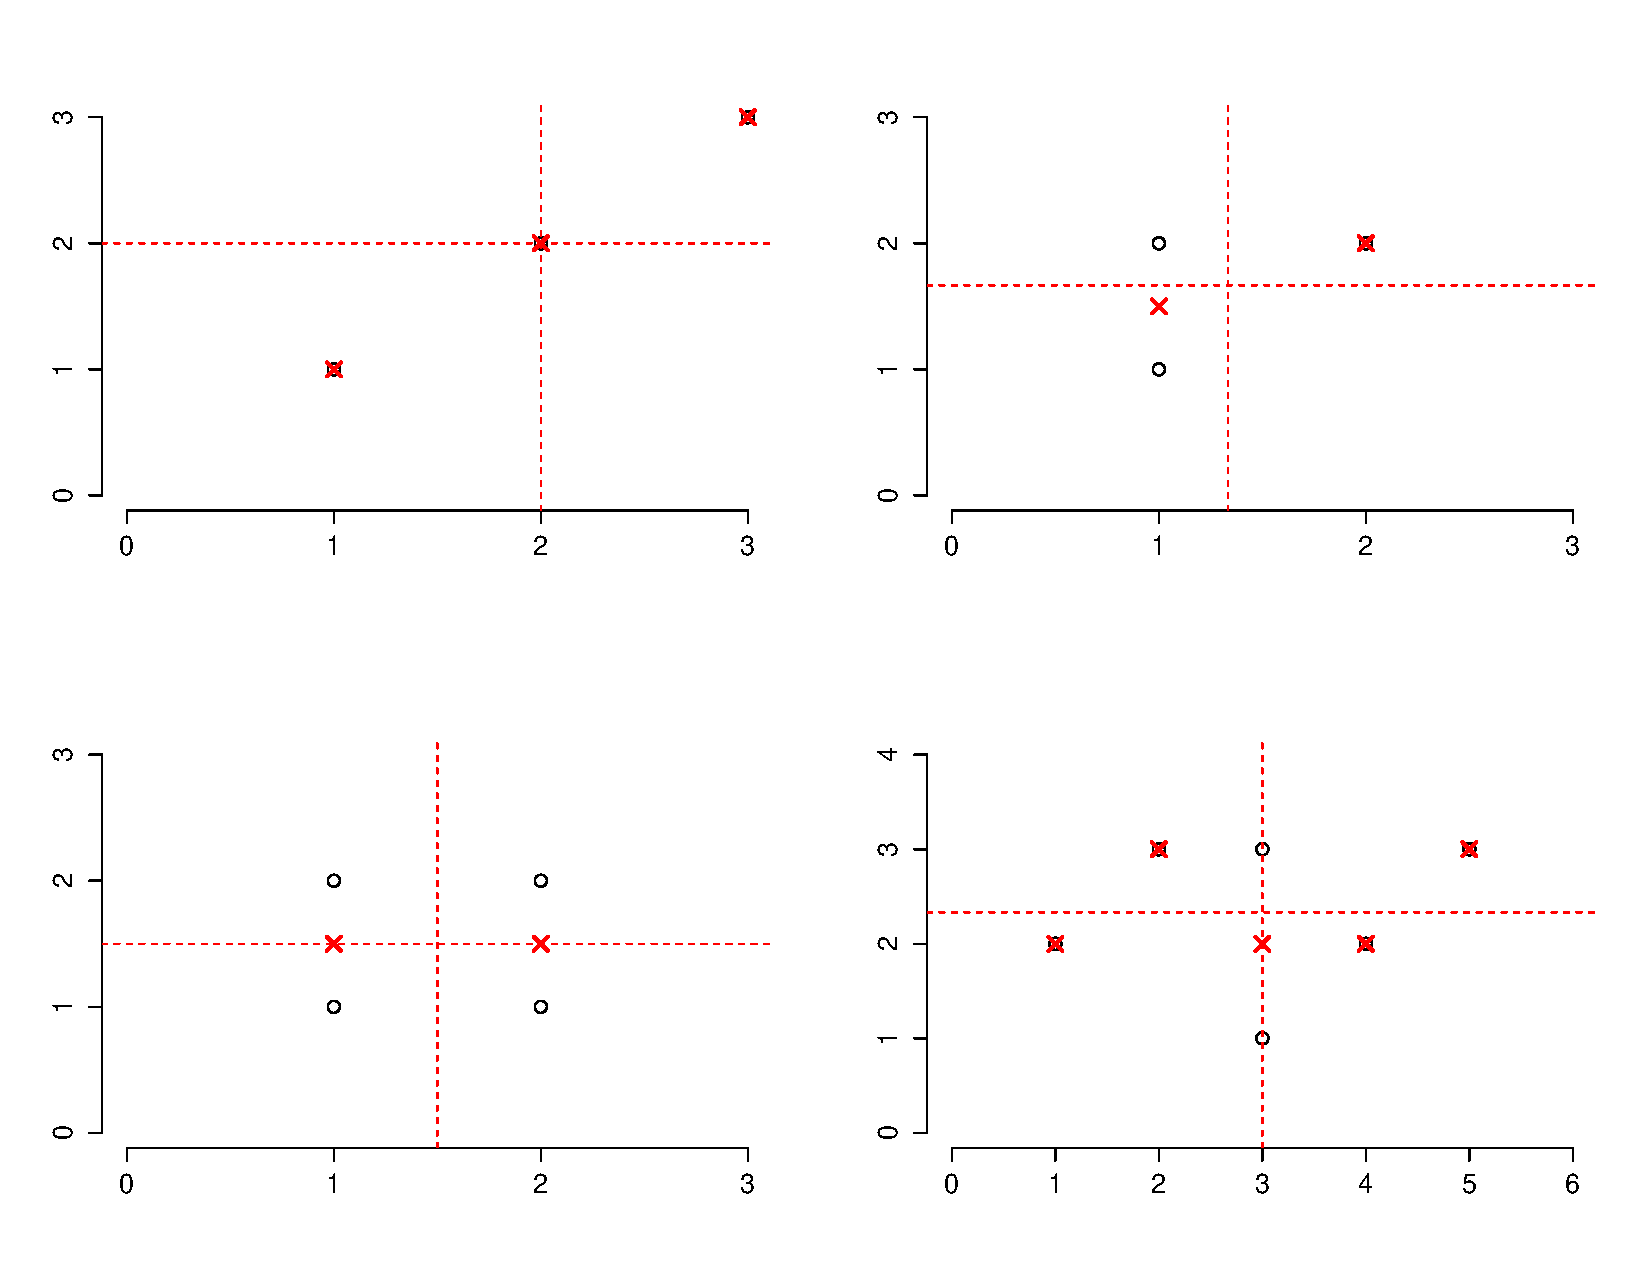
\includegraphics[scale = 0.4]{./images/Gelman_example3}}


\end{frame}

%%%%%%%%%%%%%%%%%%%%%%%%%%%%%%%%%%%%%%%%

\begin{frame}

\centering{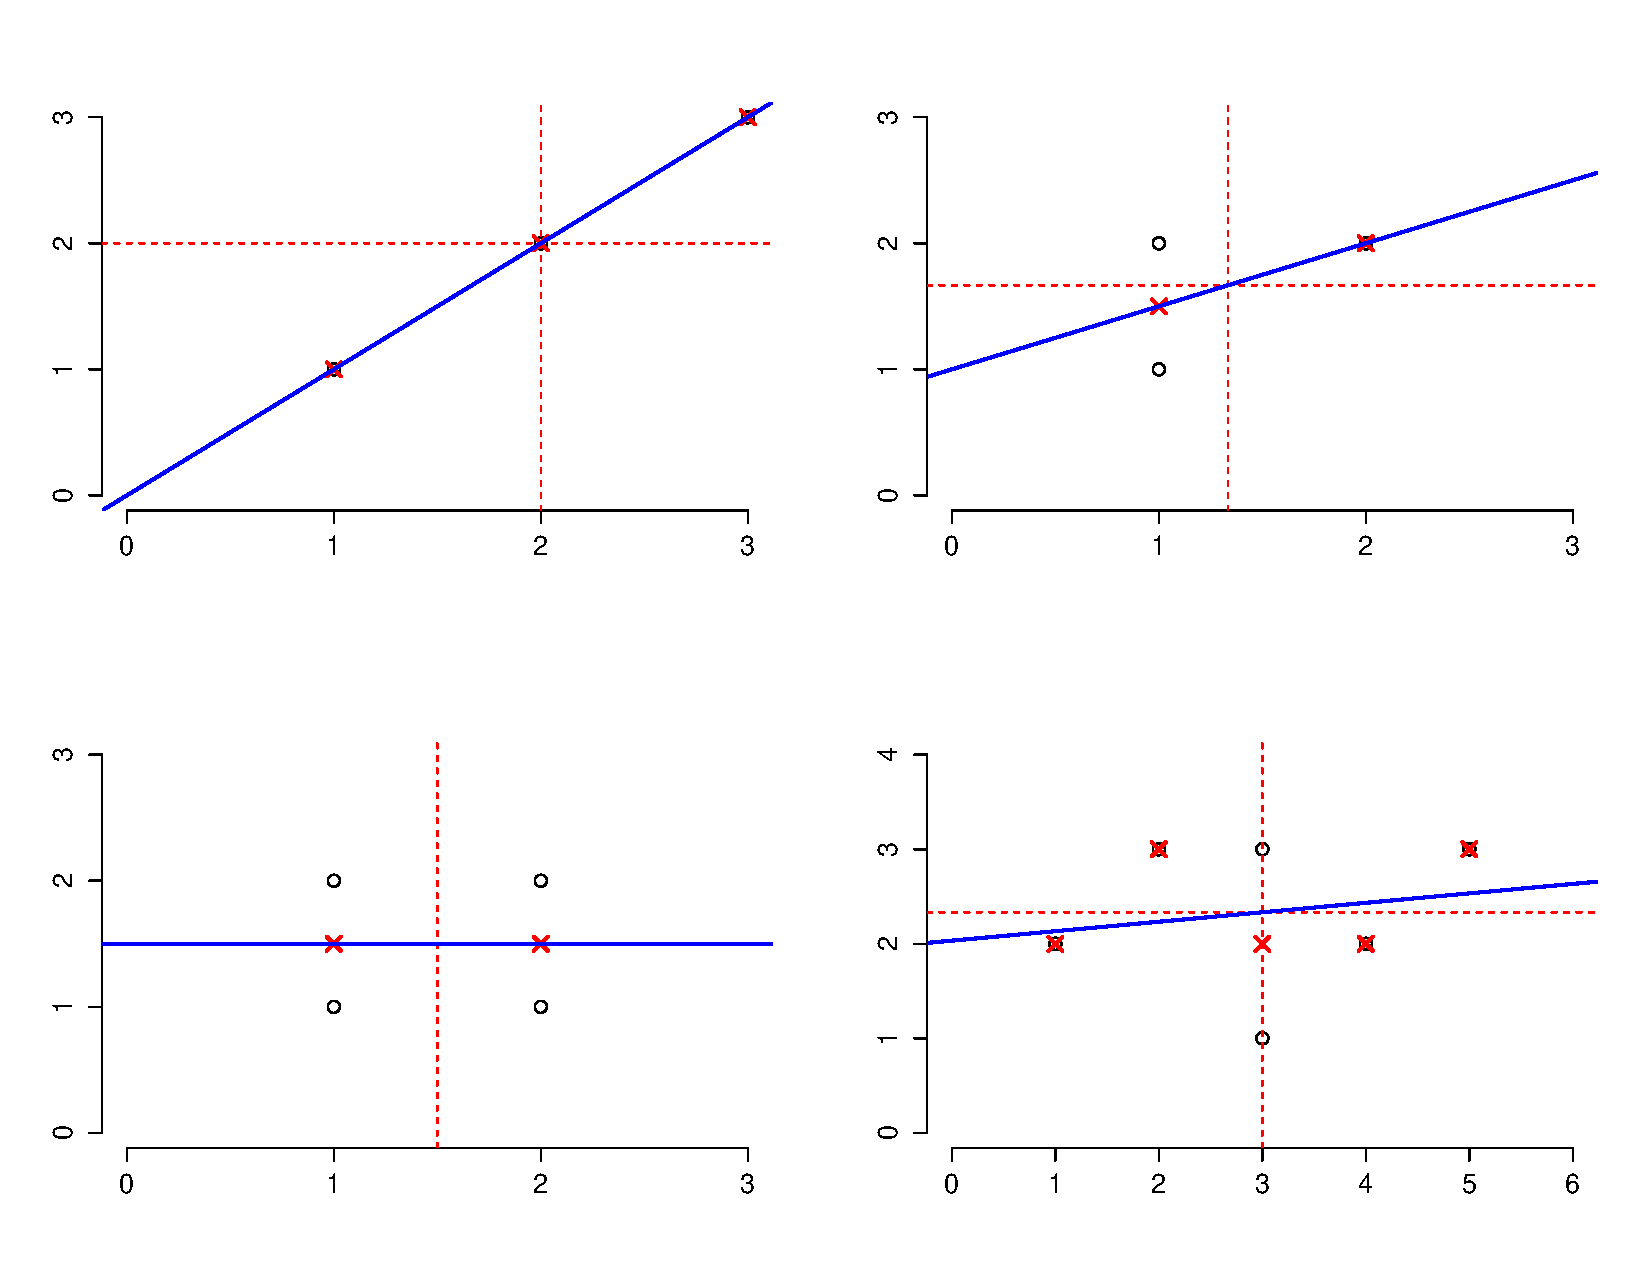
\includegraphics[scale = 0.4]{./images/Gelman_example4}}


\end{frame}

%%%%%%%%%%%%%%%%%%%%%%%%%%%%%%%%%%%%%%%%

\begin{frame}

\centering \Huge But How to Do this Formally?


\end{frame}
%%%%%%%%%%%%%%%%%%%%%%%%%%%%%%%%%%%%%%%%
\begin{frame}
\frametitle{Least Squares Regression -- Predict Using a Line}

\begin{block}{The Prediction}
Predict score $\hat{y} = a + b x$ on 2nd midterm if you scored $x$ on 1st
\end{block}

\begin{block}{How to choose $(a,b)$?}
  Linear regression chooses the slope ($b$) and intercept ($a$) that \alert{minimize the sum of squared vertical deviations}
$\displaystyle\sum_{i = 1}^n d_i^2 = \sum_{i=1}^n (y_i - a - b x_i)^2$
\end{block}

\begin{block}{Why Squared Deviations?}
\end{block}
\end{frame}
%%%%%%%%%%%%%%%%%%%%%%%%%%%%%%%%%%%%%%%%
\begin{frame}
	\frametitle{Important Point About Notation}
  $$\boxed{\underset{a,b}{\mbox{minimize }}\sum_{i = 1}^n d_i^2 = \sum_{i=1}^n (y_i - a - b x_i)^2}$$
			$$\boxed{\hat{y} = a + bx}$$
		\begin{itemize}
		\item $(x_i, y_i)_{i=1}^n$ are the \alert{observed data}
		\item $\widehat{y}$ is our \alert{prediction} for a given value of $x$
		\item Neither $x$ nor $\widehat{y}$ needs to be in out dataset!
	\end{itemize}
\end{frame}
%%%%%%%%%%%%%%%%%%%%%%%%%%%%%%%%%%%%%%%%%
%\begin{frame}
%\frametitle{Key Point}
%	\begin{itemize}
%\item Each choice of $a,b$ defines a line \pause
%\item Given the data, each line defines collection of vertical devs.\
%	$d_i = y_i - a - bx_i$ for $i=1, \hdots, n$ \pause
%\item Each collection of vertical devs.\ gives sum of squares $\sum_{i=1}^n d_i^2$ \pause
%\item We choose $a,b$ to minimize $\sum_{i=1}^n d_i^2$
%\end{itemize}
%\end{frame}
%
%
%%%%%%%%%%%%%%%%%%%%%%%%%%%%%%%%%%%%%%%%%
\begin{frame}
\begin{figure}
	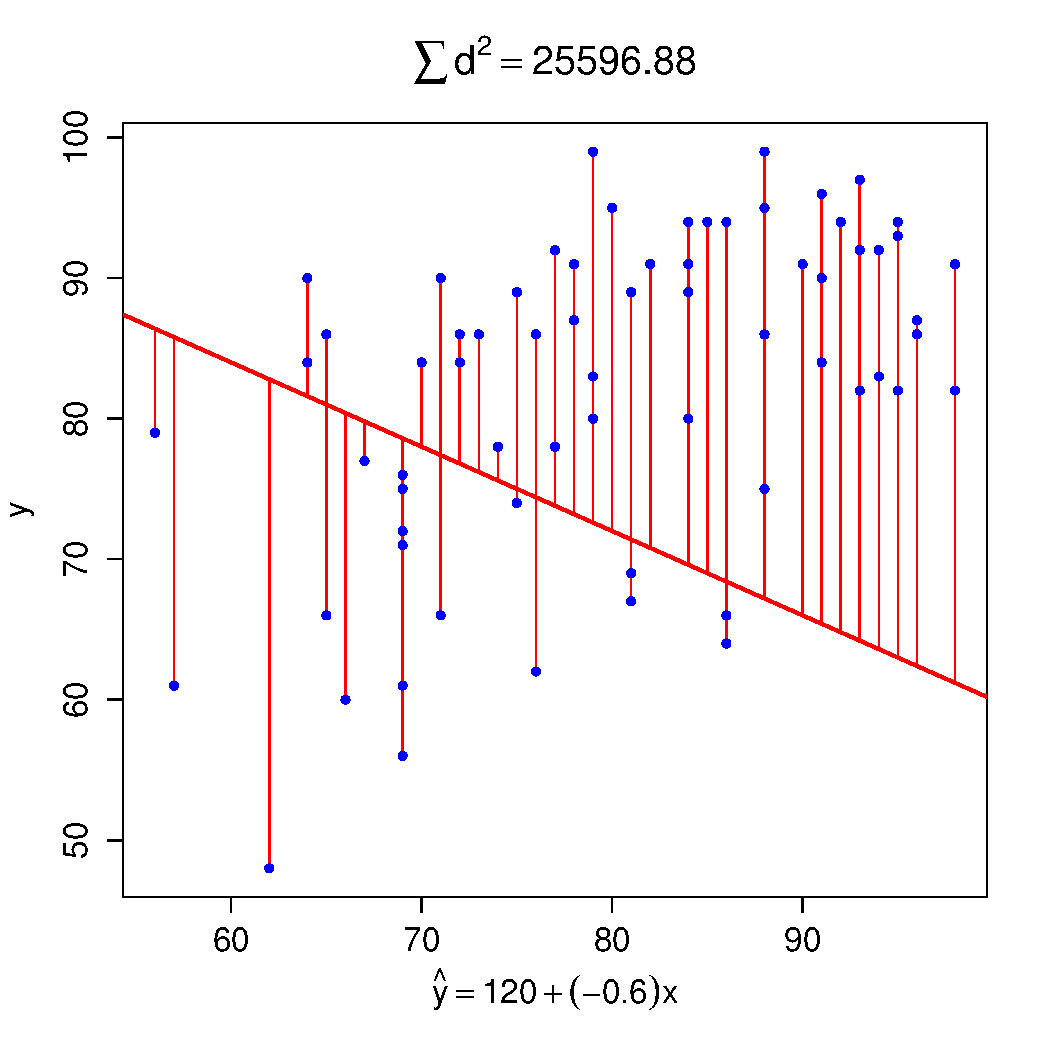
\includegraphics[scale = 0.48]{./images/SS1}
\end{figure}
\end{frame}
%%%%%%%%%%%%%%%%%%%%%%%%%%%%%%%%%%%%%%%%
\begin{frame}
\begin{figure}
	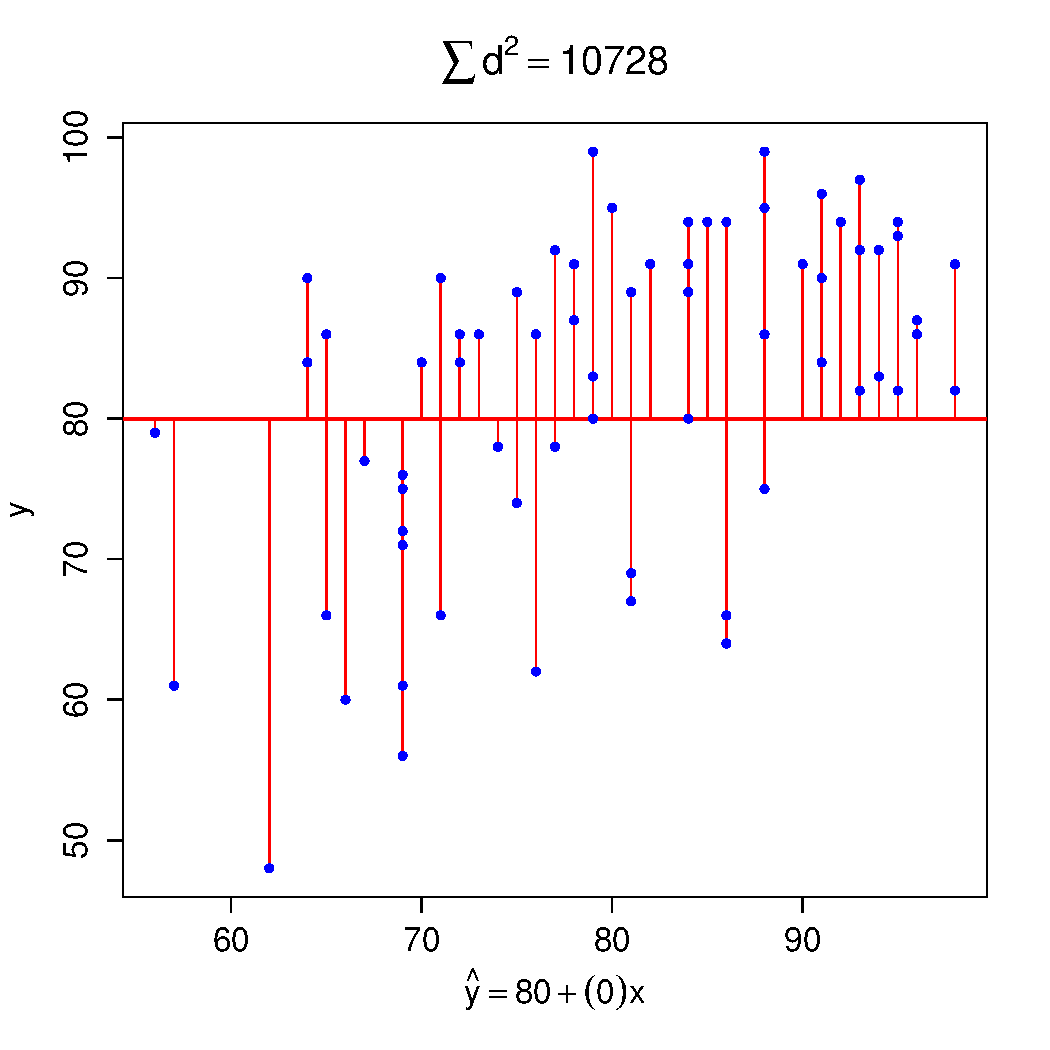
\includegraphics[scale = 0.48]{./images/SS2}
\end{figure}
\end{frame}
%%%%%%%%%%%%%%%%%%%%%%%%%%%%%%%%%%%%%%%%
\begin{frame}
\begin{figure}
	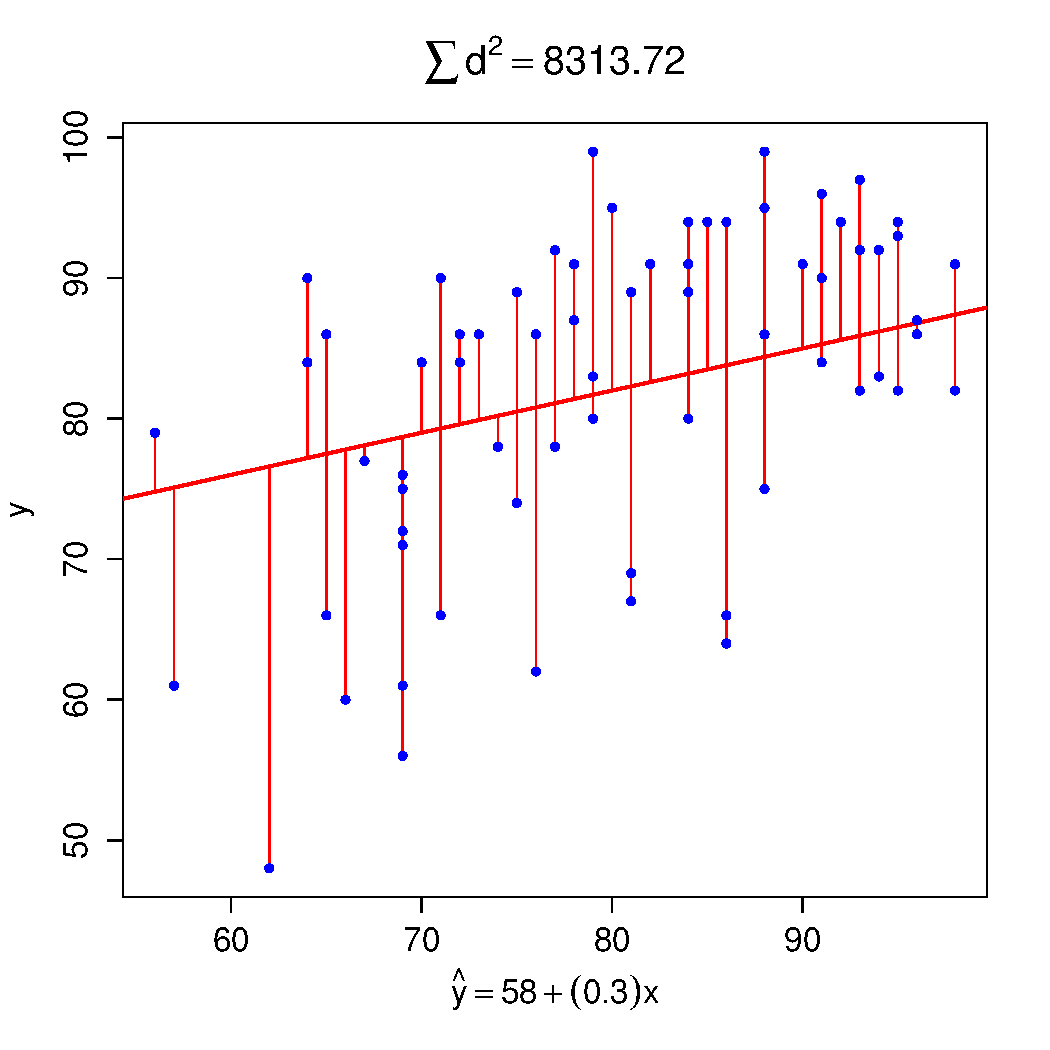
\includegraphics[scale = 0.48]{./images/SS3}
\end{figure}
\end{frame}
%%%%%%%%%%%%%%%%%%%%%%%%%%%%%%%%%%%%%%%%
\begin{frame}
\begin{figure}
	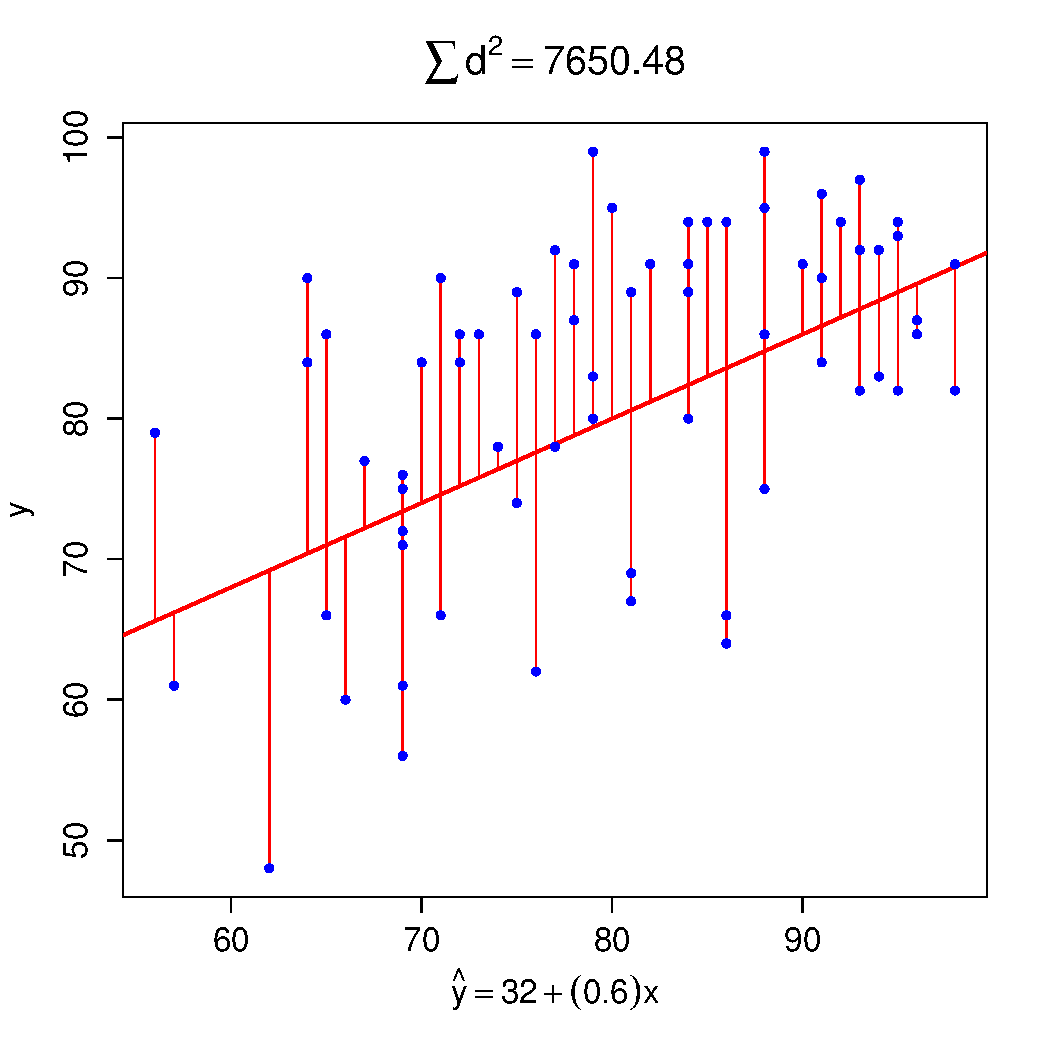
\includegraphics[scale = 0.48]{./images/SS4}
\end{figure}
\end{frame}
%%%%%%%%%%%%%%%%%%%%%%%%%%%%%%%%%%%%%%%%
\begin{frame}
\frametitle{Prediction given 89 on Midterm 1? \hfill 
\includegraphics[scale = 0.05]{./images/clicker} }
\begin{figure}
	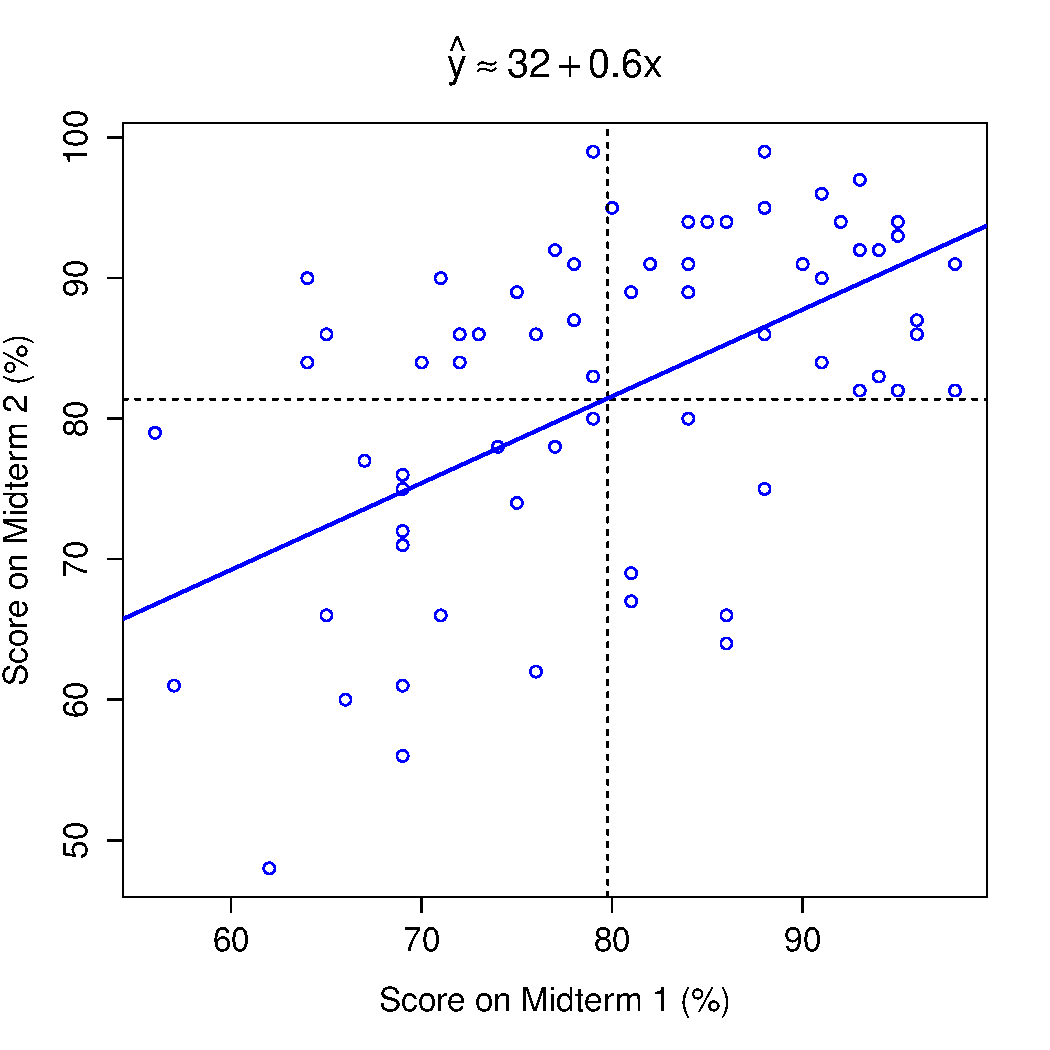
\includegraphics[scale = 0.48]{./images/midterms5}
\end{figure}
\end{frame}
%%%%%%%%%%%%%%%%%%%%%%%%%%%%%%%%%%%%%%%%
\begin{frame}
\frametitle{Prediction given 89 on Midterm 1? }
\begin{figure}
	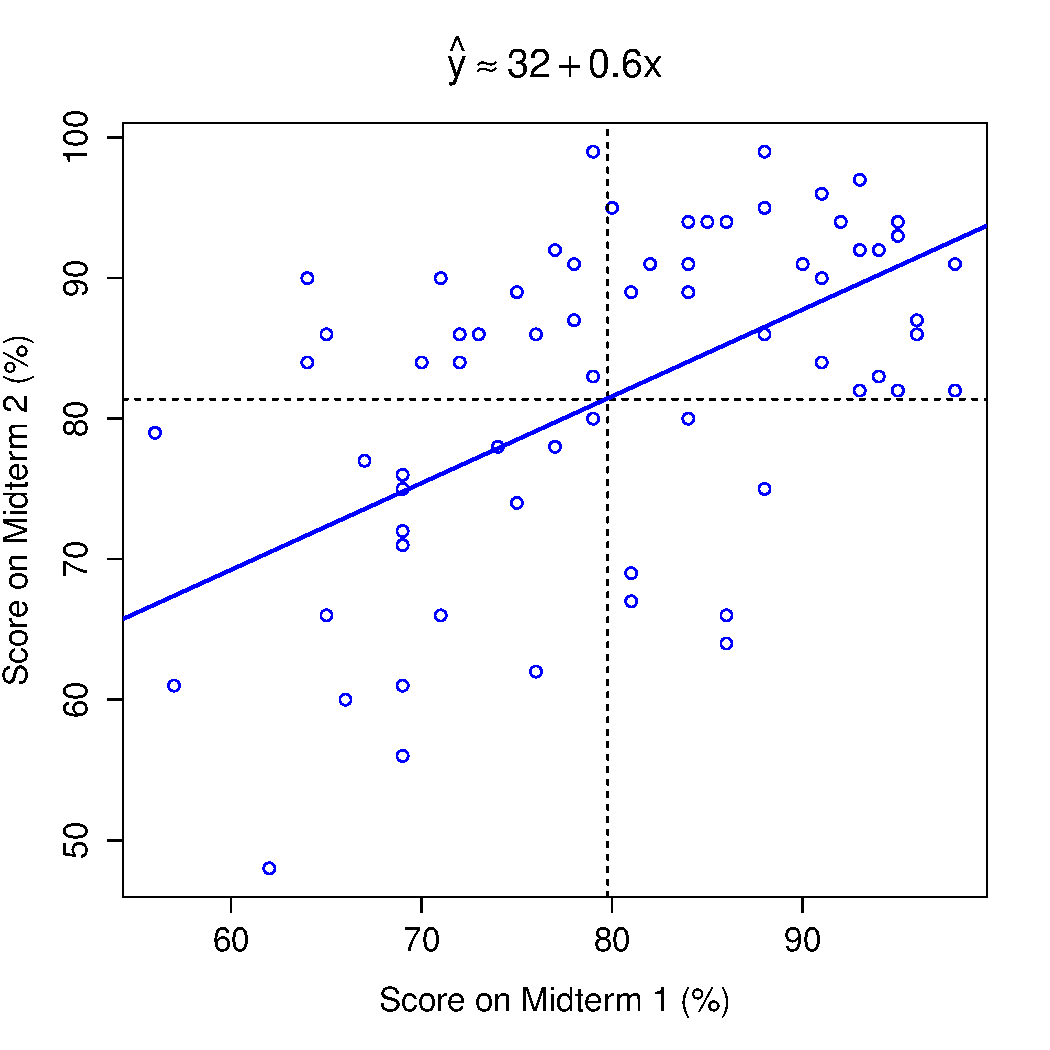
\includegraphics[scale = 0.38]{./images/midterms5}
	$$\alert{32 + 0.6 \times 89 = 32 + 53.4 = 85.4}$$
\end{figure}
\end{frame}
%%%%%%%%%%%%%%%%%%%%%%%%%%%%%%%%%%%%%%%%

\begin{frame}
\frametitle{You Need to Know How To Derive This \hfill 
\includegraphics[scale = 0.05]{./images/clicker}}
\alert{Minimize the sum of squared vertical deviations from the line:}
\begin{eqnarray*}
\min_{a,b}  \sum_{i=1}^n (y_i - a - b x_i)^2
\end{eqnarray*}
How should we proceed?
\begin{enumerate}[(a)]
	\item Differentiate with respect to $x$
	\item Differentiate with respect to $y$
	\item Differentiate with respect to $x,y$
	\item Differentiate with respect to $a,b$
	\item Can't solve this with calculus.
\end{enumerate}
\end{frame}
%%%%%%%%%%%%%%%%%%%%%%%%%%%%%%%%%%%%%%%%
\begin{frame}
\begin{block}{Objective Function}
$$\displaystyle \min_{a,b}  \sum_{i=1}^n (y_i - a - b x_i)^2$$
\end{block}
\begin{block}{FOC with respect to $a$}\pause
\begin{eqnarray*}
	-2 \sum_{i=1}^n\left(y_i - a -bx_i\right) &=& 0 \\\pause
	\sum_{i=1}^n y_i - \sum_{i=1}^n a - b\sum_{i=1}^n x_i &=& 0 \\\pause
	\frac{1}{n} \sum_{i=1}^n y_i - \frac{na}{n} -  \frac{b}{n} \sum_{i=1}^n x_i &=& 0\\\pause
	\bar{y} - a - b\bar{x} &=& 0
\end{eqnarray*}
\end{block}
\end{frame}
%%%%%%%%%%%%%%%%%%%%%%%%%%%%%%%%%%%%%%%%
\begin{frame}

\frametitle{Regression Line Goes Through the Means!}
 \Huge
\begin{equation*}\boxed{\bar{y} = a + b\bar{x}}\end{equation*}
\normalsize
\end{frame}
%%%%%%%%%%%%%%%%%%%%%%%%%%%%%%%%%%%%%%%%
\begin{frame}
  \frametitle{Substitute $a = \bar{y} - b \bar{x}$}
  \small
\begin{eqnarray*}
	\sum_{i=1}^n (y_i - a - b x_i)^2 &=& \pause\sum_{i=1}^n (y_i - \bar{y} + b\bar{x} - b x_i)^2\\
	&=&\pause\sum_{i=1}^n \left[ \left(y_i - \bar{y}\right) - b\left(x_i - \bar{x}\right) \right]^2
\end{eqnarray*}
\alert{FOC wrt $b$}
\begin{eqnarray*}\pause
	-2\sum_{i=1}^n \left[\left(y_i - \bar{y}\right) - b\left(x_i - \bar{x}\right) \right]\left(x_i - \bar{x} \right) &=& 0\\\pause
	\sum_{i=1}^n \left(y_i - \bar{y}\right)\left(x_i - \bar{x} \right) - b\sum_{i=1}^n \left(x_i - \bar{x}\right)^2 &=& 0\\ \\\pause
	b = \frac{\sum_{i=1}^n \left(y_i - \bar{y}\right)\left(x_i - \bar{x} \right)}{\sum_{i=1}^n \left(x_i - \bar{x}\right)^2}
\end{eqnarray*}
\end{frame}
%%%%%%%%%%%%%%%%%%%%%%%%%%%%%%%%%%%%%%%%
\begin{frame}
\frametitle{Simple Linear Regression}
	\begin{block}{Problem}
	$$\min_{a,b}  \sum_{i=1}^n (y_i - a - b x_i)^2$$
\end{block}
\begin{block}{Solution}
	\begin{eqnarray*}
		b &=& \frac{\sum_{i=1}^n \left(y_i - \bar{y}\right)\left(x_i - \bar{x} \right)}{\sum_{i=1}^n \left(x_i - \bar{x}\right)^2}\\ \\
		a &=& \bar{y} - b\bar{x}
	\end{eqnarray*}
\end{block}
\end{frame}

%%%%%%%%%%%%%%%%%%%%%%%%%%%%%%%%%%%%%%%%
\begin{frame}
	\frametitle{Relating Regression to Covariance and Correlation}
		$$b = \frac{\sum_{i=1}^n \left(y_i - \bar{y}\right)\left(x_i - \bar{x} \right)}{\sum_{i=1}^n \left(x_i - \bar{x}\right)^2} = \frac{\frac{1}{n-1}\sum_{i=1}^n \left(y_i - \bar{y}\right)\left(x_i - \bar{x} \right)}{\frac{1}{n-1}\sum_{i=1}^n \left(x_i - \bar{x}\right)^2} = \frac{s_{xy}}{s_x^2}$$
		
		$$r = \frac{s_{xy}}{s_x s_y} = b \frac{s_x}{s_y}$$
		
\end{frame}
%%%%%%%%%%%%%%%%%%%%%%%%%%%%%%%%%%%%%%%%
\begin{frame}
\frametitle{Comparing Regression, Correlation and Covariance}

\begin{block}{Units}
Correlation is unitless, covariance and regression coefficients ($a, b$) are not. (What are the units of these?)
\end{block}


\begin{block}{Symmetry}
Correlation and covariance are symmetric, regression isn't. (Switching $x$ and $y$ axes changes the slope and intercept.)
\end{block}

\begin{block}{On the Homework}
Regression with z-scores rather than raw data gives $a=0, b = r_{xy}$
\end{block}

\end{frame}
%%%%%%%%%%%%%%%%%%%%%%%%%%%%%%%%%%%%%%%%

\begin{frame}
\frametitle{
\includegraphics[scale = 0.05]{./images/clicker}}

$\begin{array}{ccccc} s_{xy} = 6,&s_x = 5,& s_y = 2,& \bar{x} = 68,& \bar{y} = 21\end{array}$
\begin{columns}[c]
\column{2.5in}
What is the sample correlation between height ($x$) and handspan ($y$)?
\column{1.8in}
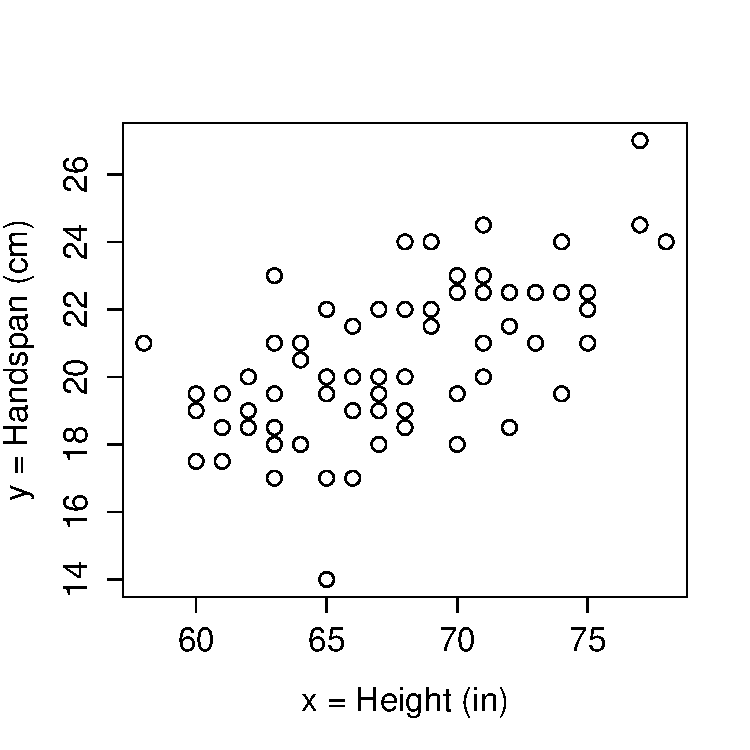
\includegraphics[scale = 0.4]{./images/height_handspan1}
\end{columns}
\alert{$$\phantom{r = \frac{s_{xy}}{s_x s_y} = \frac{6}{4.5\times 2.2} \approx 0.6}$$}
\end{frame}
%%%%%%%%%%%%%%%%%%%%%%%%%%%%%%%%%%%%%%%%
\begin{frame}
\frametitle{
\includegraphics[scale = 0.05]{./images/clicker}}
$\begin{array}{ccccc} s_{xy} = 6,&s_x = 5,& s_y = 2,& \bar{x} = 68,& \bar{y} = 21\end{array}$
\begin{columns}[c]
\column{2.5in}
What is the sample correlation between height ($x$) and handspan ($y$)?
\column{1.8in}
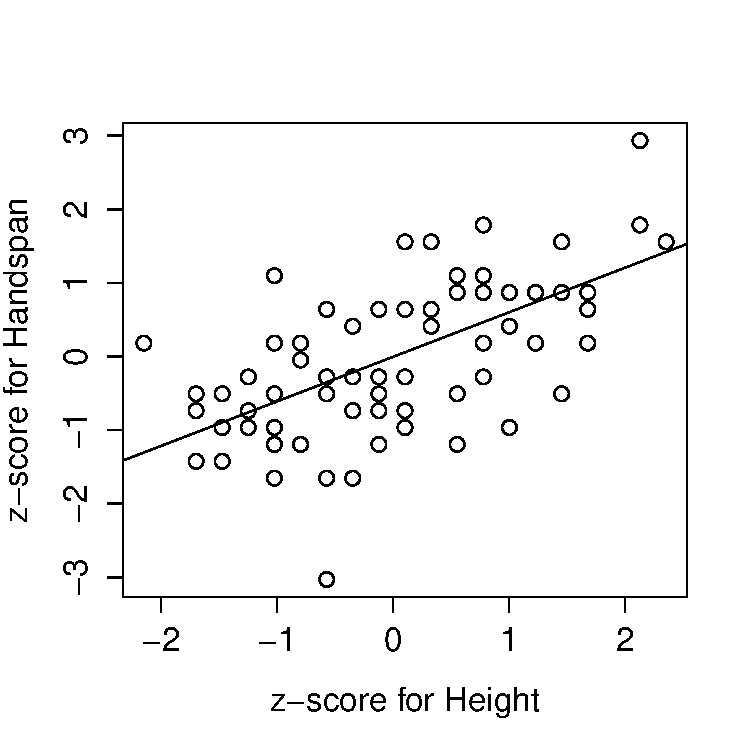
\includegraphics[scale = 0.4]{./images/height_handspan_zline}
\end{columns}
\alert{$$r = \frac{s_{xy}}{s_x s_y} = \frac{6}{5\times 2} = 0.6$$}
\end{frame}
%%%%%%%%%%%%%%%%%%%%%%%%%%%%%%%%%%%%%%%%
\begin{frame}
\frametitle{
\includegraphics[scale = 0.05]{./images/clicker}}
$\begin{array}{ccccc} s_{xy} = 6,&s_x = 5,& s_y = 2,& \bar{x} = 68,& \bar{y} = 21\end{array}$
\begin{columns}[c]
\column{2.5in}
What is the value of $b$ for the regression: $$\hat{y}=a+bx$$
where $x$ is height and $y$ is handspan?
\column{1.8in}
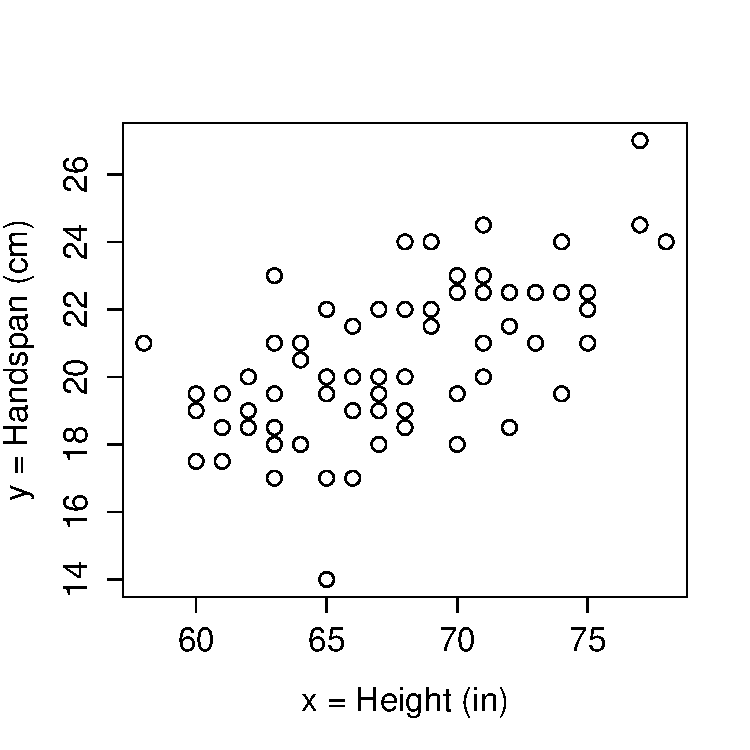
\includegraphics[scale = 0.4]{./images/height_handspan1}
\end{columns}
\alert{$$\phantom{b = \frac{s_{xy}}{s_x^2} = \frac{6}{(4.5)^2} = 6/20.25 \approx 0.3}$$}
\end{frame}
%%%%%%%%%%%%%%%%%%%%%%%%%%%%%%%%%%%%%%%%
\begin{frame}
\frametitle{
\includegraphics[scale = 0.05]{./images/clicker}}
$\begin{array}{ccccc} s_{xy} = 6,&s_x = 5,& s_y = 2,& \bar{x} = 68,& \bar{y} = 21\end{array}$
\begin{columns}[c]
\column{2.5in}
What is the value of $b$ for the regression: $$\hat{y}=a+bx$$
where $x$ is height and $y$ is handspan?
\column{1.8in}
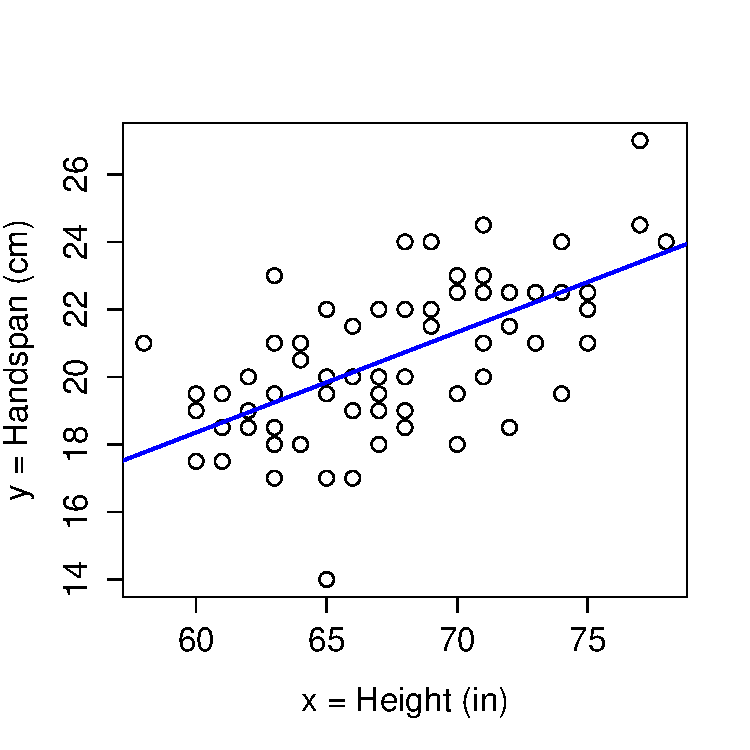
\includegraphics[scale = 0.4]{./images/height_handspan2}
\end{columns}
\alert{$$b = \frac{s_{xy}}{s_x^2} = \frac{6}{5^2} = 6/25 = 0.24 $$}
\end{frame}
%%%%%%%%%%%%%%%%%%%%%%%%%%%%%%%%%%%%%%%%
\begin{frame}
\frametitle{
\includegraphics[scale = 0.05]{./images/clicker}}
$\begin{array}{ccccc} s_{xy} = 6,&s_x = 5,& s_y = 2,& \bar{x} = 68,& \bar{y} = 21\end{array}$
\begin{columns}[c]
\column{2.5in}
What is the value of $a$ for the regression: $$\hat{y}=a+bx$$
where $x$ is height and $y$ is handspan? (prev.\ slide $b = 0.24$)
\column{1.8in}
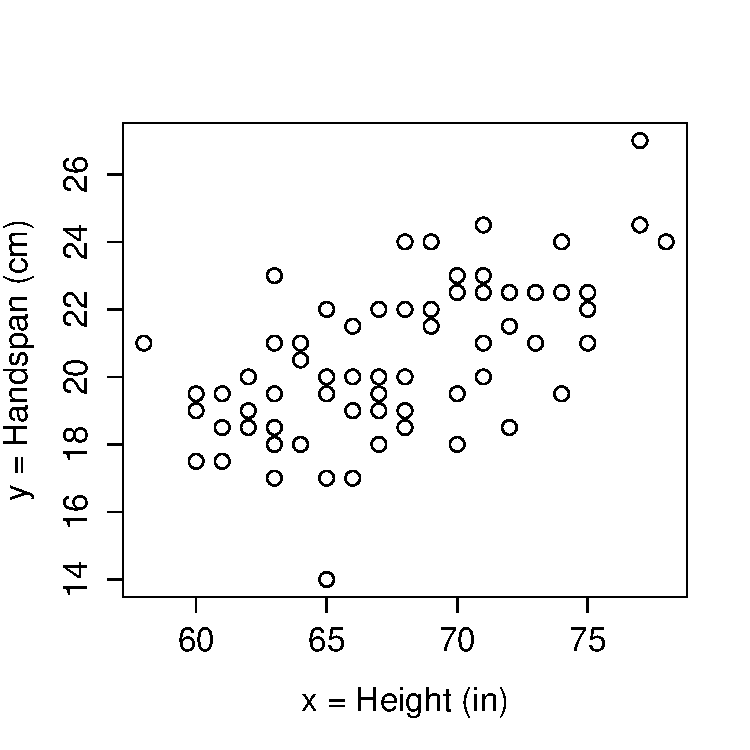
\includegraphics[scale = 0.4]{./images/height_handspan1}
\end{columns}
\alert{$$\phantom{a = \bar{y} - b \bar{x} = 20.6 - 0.297 \times 67.6 \approx 0.5}$$}
\end{frame}
%%%%%%%%%%%%%%%%%%%%%%%%%%%%%%%%%%%%%%%%
\begin{frame}
\frametitle{
\includegraphics[scale = 0.05]{./images/clicker}}
$\begin{array}{ccccc} s_{xy} = 6,&s_x = 5,& s_y = 2,& \bar{x} = 68,& \bar{y} = 21\end{array}$
\begin{columns}[c]
\column{2.5in}
What is the value of $a$ for the regression: $$\hat{y}=a+bx$$
where $x$ is height and $y$ is handspan? (prev.\ slide $b = 0.24$)
\column{1.8in}
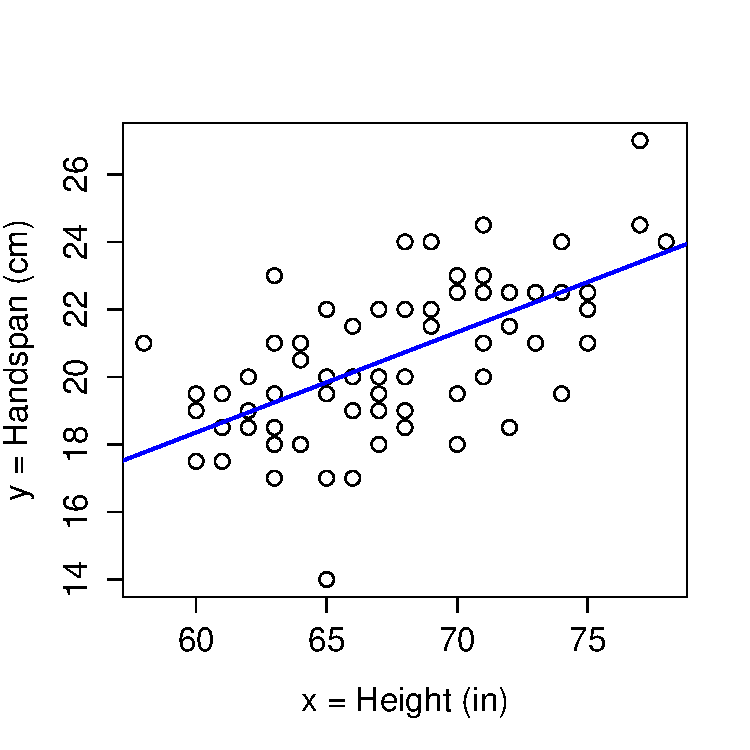
\includegraphics[scale = 0.4]{./images/height_handspan2}
\end{columns}
\alert{$$a = \bar{y} - b \bar{x} = 21 - 0.24 \times 68 = 4.68 $$}
\end{frame}
%%%%%%%%%%%%%%%%%%%%%%%%%%%%%%%%%%%%%%%%
\begin{frame}
\frametitle{
\includegraphics[scale = 0.05]{./images/clicker}}
\alert{$\begin{array}{ccccc} s_{xy} = 6,&s_y = 5,& s_x = 2,& \bar{y} = 68,& \bar{x} = 21\end{array}$}
\begin{columns}[c]
\column{2.5in}
What is the value of $b$ for the regression: $$\hat{y}=a+bx$$
where \alert{$x$ is handspan and $y$ is height? }
\column{1.8in}
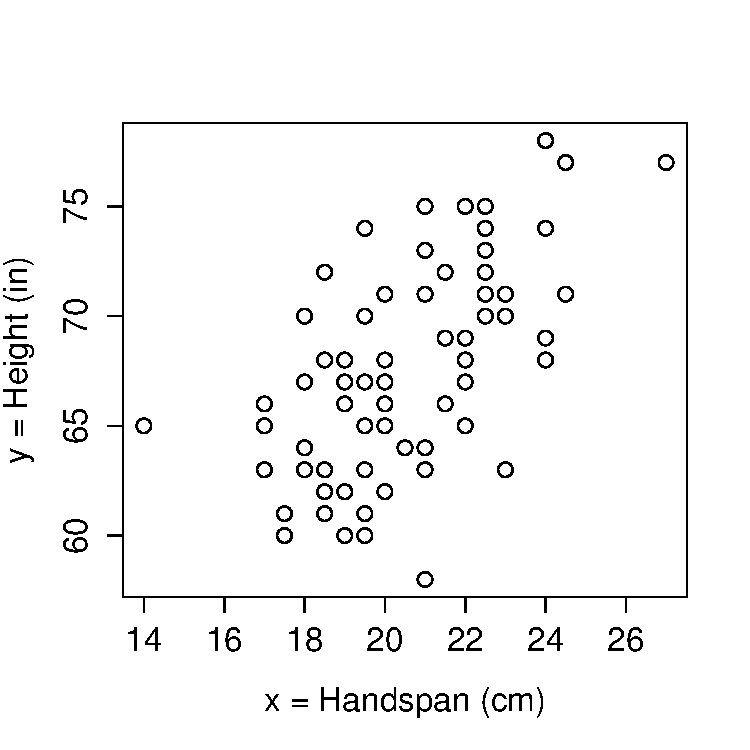
\includegraphics[scale = 0.4]{./images/handspan_height}
\end{columns}
\alert{$$\phantom{b = \frac{s_{xy}}{s_x^2} = 6 /2.2^2 \approx 1.2}$$}
\end{frame}
%%%%%%%%%%%%%%%%%%%%%%%%%%%%%%%%%%%%%%%%
\begin{frame}
\frametitle{
\includegraphics[scale = 0.05]{./images/clicker}}
\alert{$\begin{array}{ccccc} s_{xy} = 6,&s_y = 5,& s_x = 2,& \bar{y} = 68,& \bar{x} = 21\end{array}$}
\begin{columns}[c]
\column{2.5in}
What is the value of $b$ for the regression: $$\hat{y}=a+bx$$
where \alert{$x$ is handspan and $y$ is height? }
\column{1.8in}
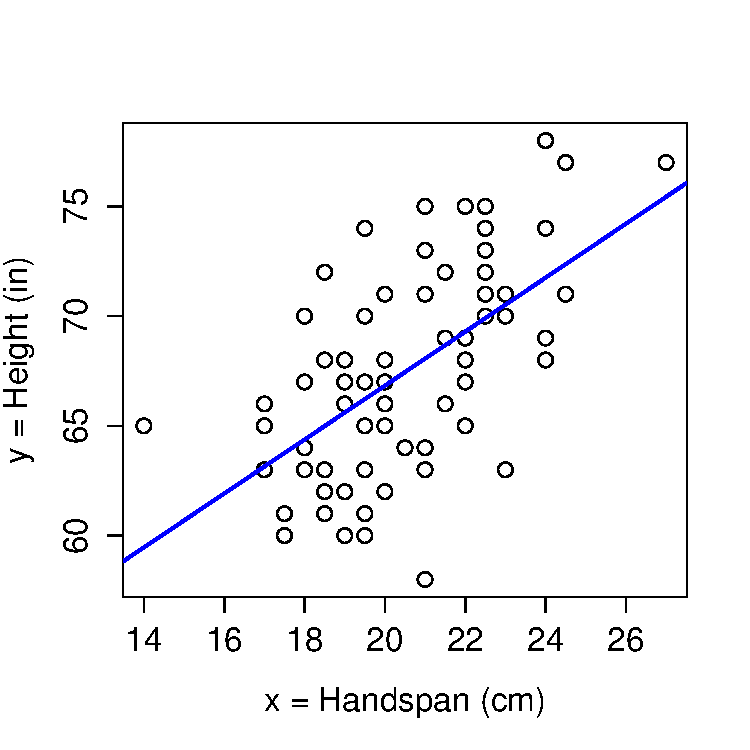
\includegraphics[scale = 0.4]{./images/handspan_height2}
\end{columns}
\alert{$$b = \frac{s_{xy}}{s_x^2} = 6 /2^2 = 1.5 $$}
\end{frame}
%%%%%%%%%%%%%%%%%%%%%%%%%%%%%%%%%%%%%%%%
\begin{frame}

\begin{alertblock}{EXTREMELY IMPORTANT}
	\begin{itemize}
		\item Regression, Covariance and Correlation: linear association.
		\item Linear association $\neq$ causation. 
		\item Linear is not the only kind of association!
	\end{itemize}
\end{alertblock}

\centering{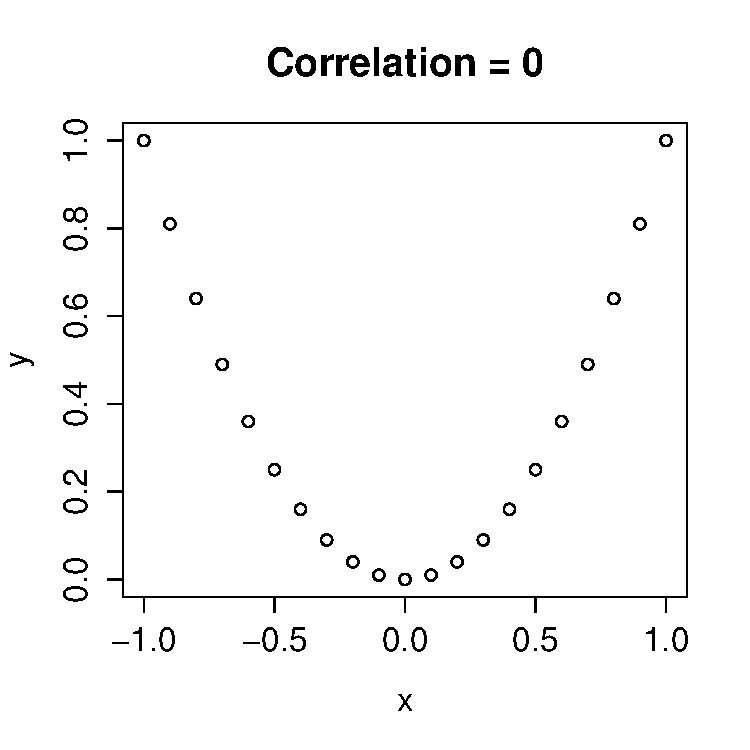
\includegraphics[scale = 0.45]{./images/zero_corr}}

\end{frame}

%%%%%%%%%%%%%%%%%%%%%%%%%%%%%%%%%%%%%%%%
\begin{frame}
  \frametitle{Regression to the Mean and the Regression Fallacy}

  \alert{Please read Chapter 17 of ``Thinking Fast and Slow'' by Daniel Kahnemann which I have posted on Piazza. This reading is fair game on an exam or quiz.}
\end{frame}
%%%%%%%%%%%%%%%%%%%%%%%%%%%%%%%%%%%%%%%%
\begin{frame}

\centering{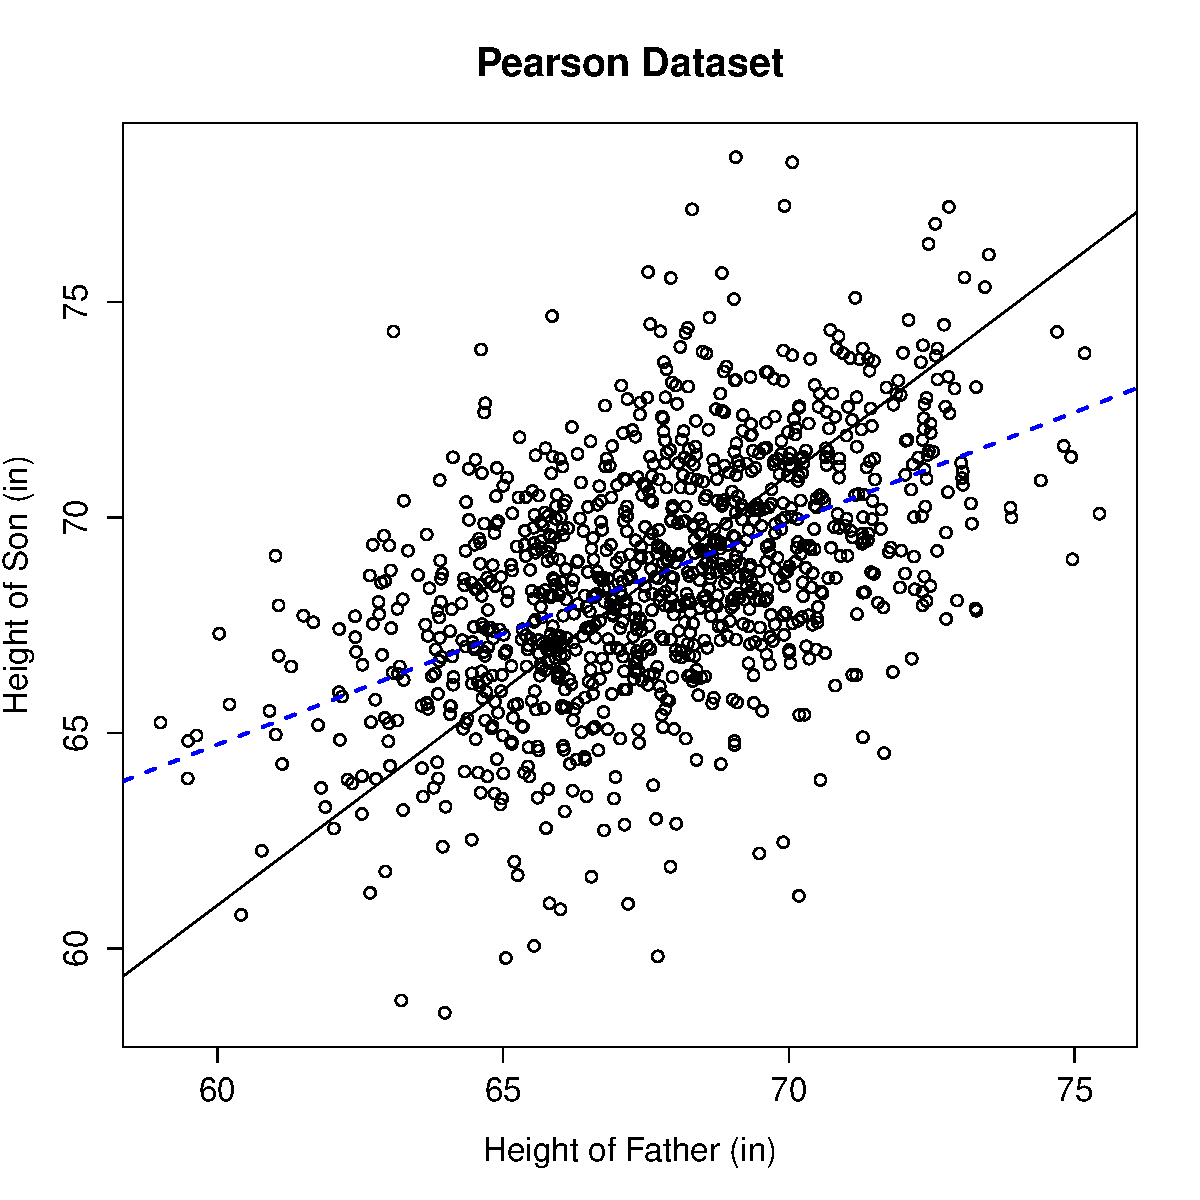
\includegraphics[scale = 0.46]{./images/pearson}}


\end{frame}

%%%%%%%%%%%%%%%%%%%%%%%%%%%%%%%%%%%%%%%%
%\begin{frame}
%\frametitle{
\includegraphics[scale = 0.05]{./images/clicker}}
%
%Suppose a father is very short compared to other fathers (very negative z-score). Would you expect his son to be:
%	\begin{enumerate}[(a)]
%\item Shorter
%\item About as short
%\item Taller
%\end{enumerate}
%\end{frame}

%%%%%%%%%%%%%%%%%%%%%%%%%%%%%%%%%%%%%%%%
%\begin{frame}
%
%\centering{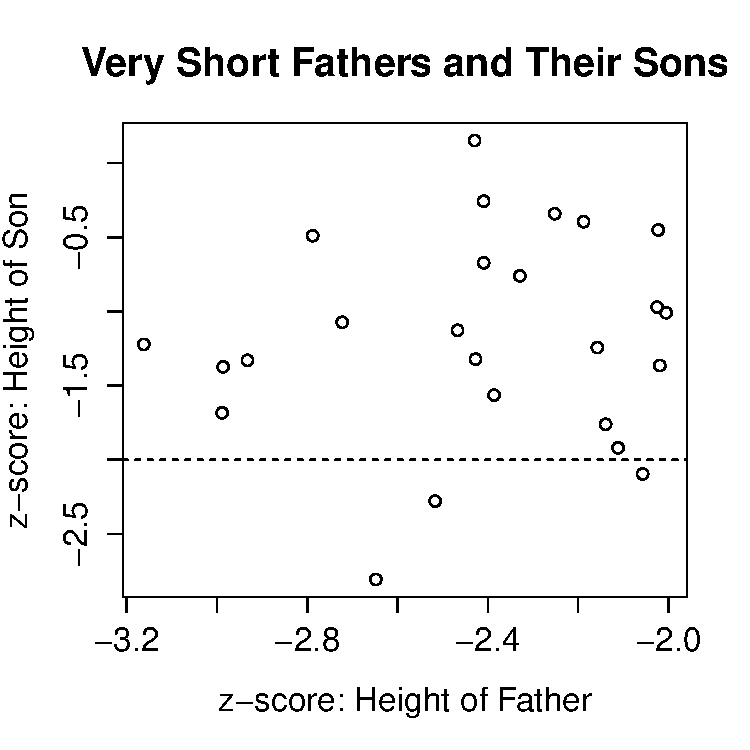
\includegraphics[scale = 0.65]{./images/short_father}}
%
%
%\end{frame}
%
%%%%%%%%%%%%%%%%%%%%%%%%%%%%%%%%%%%%%%%%%
%
%
%\begin{frame}
%
%\centering{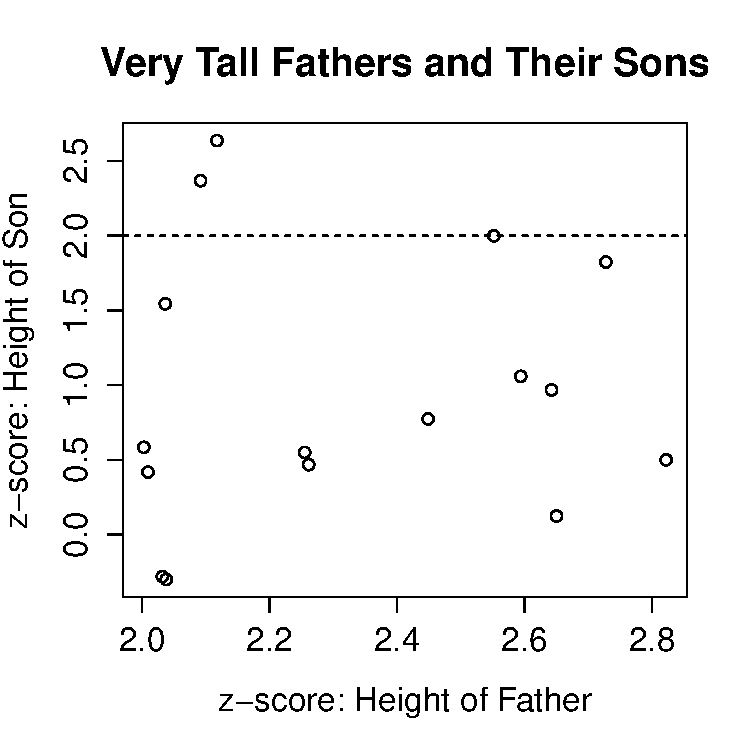
\includegraphics[scale = 0.65]{./images/tall_father}}
%
%
%\end{frame}
%
%%%%%%%%%%%%%%%%%%%%%%%%%%%%%%%%%%%%%%%%%
%
%
%\begin{frame}
%
%\centering{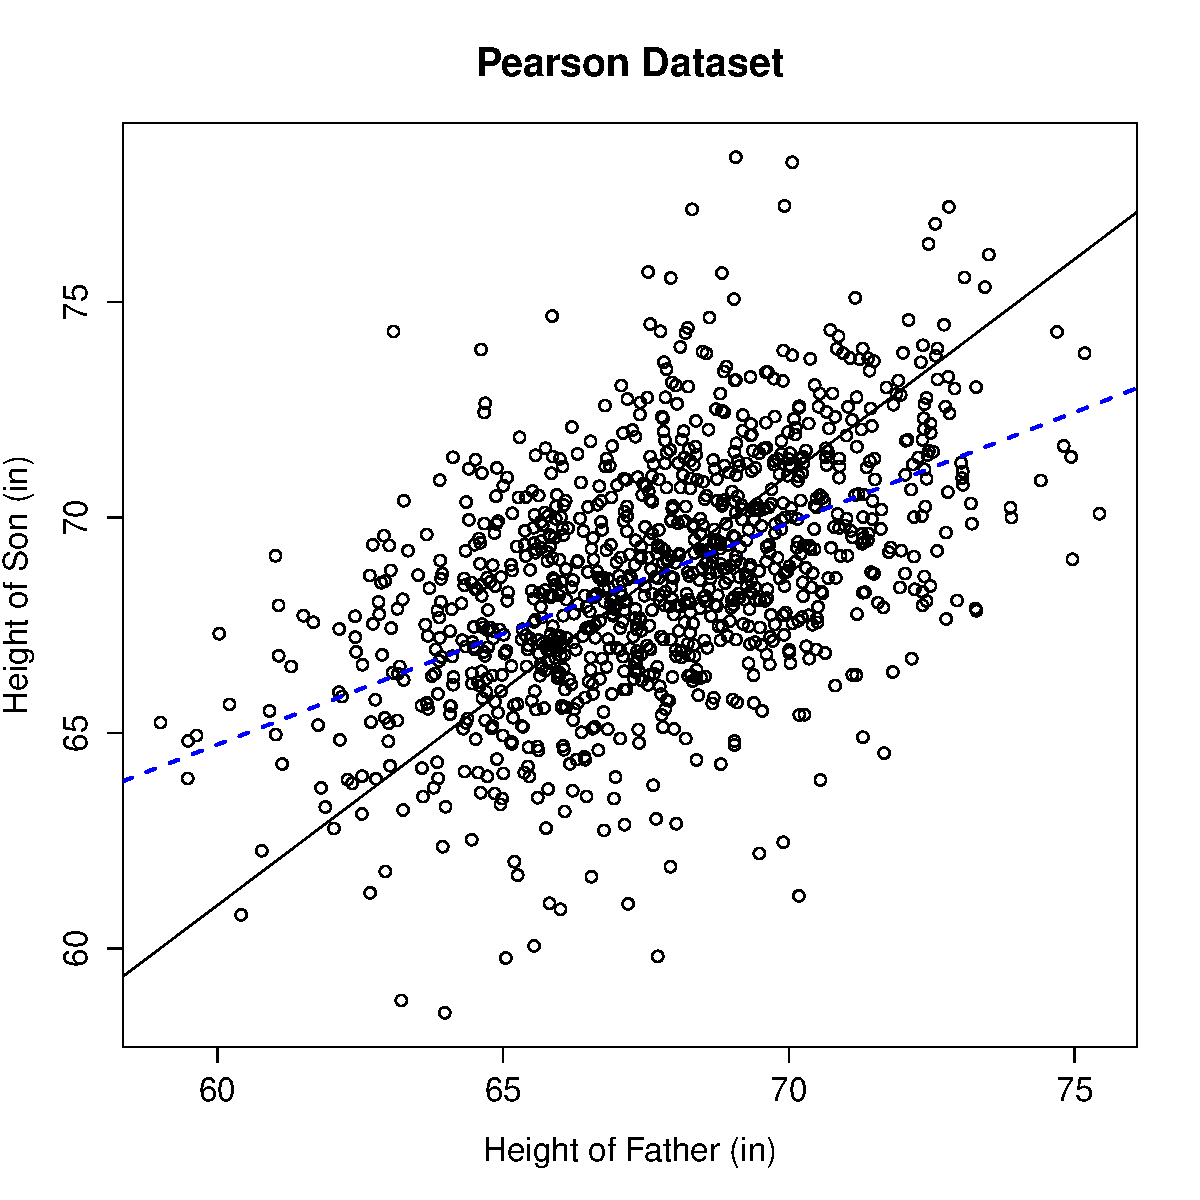
\includegraphics[scale = 0.46]{./images/pearson}}
%
%
%\end{frame}
%
%%%%%%%%%%%%%%%%%%%%%%%%%%%%%%%%%%%%%%%%

\begin{frame}
\frametitle{Regression to the Mean}

\begin{block}{Skill and Luck / Genes and Random Environmental Factors}\end{block}


\begin{block}{Unless $r_{xy}=1$, There Is Regression to the Mean}
$$\frac{\hat{y} - \bar{y}}{{s_y}} = r_{xy} \frac{x - \bar{x}}{s_x}$$
\end{block}

\begin{alertblock}{Least-squares Prediction $\hat{y}$ closer to $\bar{y}$ than $x$ is to $\bar{x}$}
\end{alertblock}
You will derive the above formula in this week's homework.
\end{frame}
%%%%%%%%%%%%%%%%%%%%%%%%%%%%%%%%%%%%%%%%
%\begin{frame}
%\frametitle{Regression Fallacy}
%\framesubtitle{For More, See the Document Posted on Piazza}
%\begin{block}{Pre-test}
%Which students are strongest, which are weakest?
%\end{block}
%
%\begin{block}{Intervention} Put the best performing in an enrichment program and the worst performing in a remedial class
%\end{block}
%
%\begin{block}{Post-test}
%The weak students did better than on their first test, but the strong students did \emph{worse}.
%\end{block}
%
%\begin{block}{Mistaken Conclusion}
%Remedial classes are beneficial, enrichment programs are harmful
%\end{block}
%\end{frame}
%%%%%%%%%%%%%%%%%%%%%%%%%%%%%%%%%%%%%%%%
\begin{frame}
  \frametitle{Next Up: Basic Probability}
  Please do the following before our next class:
      \vspace{1em}
  \begin{enumerate}
    \item Complete the ``Odd Questions'' quiz posted on Piazza \texttt{OddQuestions.pdf} -- we'll be discussing these in class.
      \vspace{1em}
    \item If you're rusty on permutations, combinations, etc. from High School math, read this review \footnotesize \url{http://ditraglia.com/Econ103Public/ClassicalProbability.pdf}
  \end{enumerate}
\end{frame}
%%%%%%%%%%%%%%%%%%%%%%%%%%%%%%%%%%%%%%%%

\end{document}
